\section{Performance Evaluation and Analysis}\label{sec:RnD}
Following the formulation of the detector, we will evaluate its detection and localization performance against MOBF orders 1 and 2. Subsequently, we will conduct a more in-depth analysis of its structural characteristics and operational behavior under varying conditions, including an examination of the captured energy and receiver operating characteristic (ROC) curves at different signal-to-noise ratio (SNR) levels. This analysis will conclude with an overview of the expected limitations and sensitivities of the proposed detector.



\subsection{Detection and Localization}

Here, two experiments have been conducted: a real experiment in a Lake, and a simulation under more controlled conditions.

\subsubsection{Lake experiments}
We evaluated the detector on magnetic data, recorded in the lake of Bourg-Blanc, approximately 15 km northeast of Brest, in Brittany, France.

The experiment involved a USV (dimensions: 180 × 120 cm), following a predetermined path while carrying a triaxial fluxgate magnetometer, photos are shown in figure \ref{fig:experiment_setup}.

The magnetic data were acquired using an autonomous data acquisition system developed by MAPPEM Geophysics. The magnetic sensor is a 3-axis fluxgate magnetometer with a noise level of 20 pT/$\sqrt{\text{Hz}}$ at 1 Hz. The data logger is synchronized at start-up on GNSS time, and acquisition is paced by a precise oscillator with an error of about 1 s per year. The data logger records the 3 components simultaneously at 500 Hz with 32-bit resolution. For the experiment, the magnetometer was installed on the USV at a distance from major electromagnetic noise sources.

\begin{figure*}[t]
\centering
\begin{minipage}[t]{0.32\textwidth}
\centering
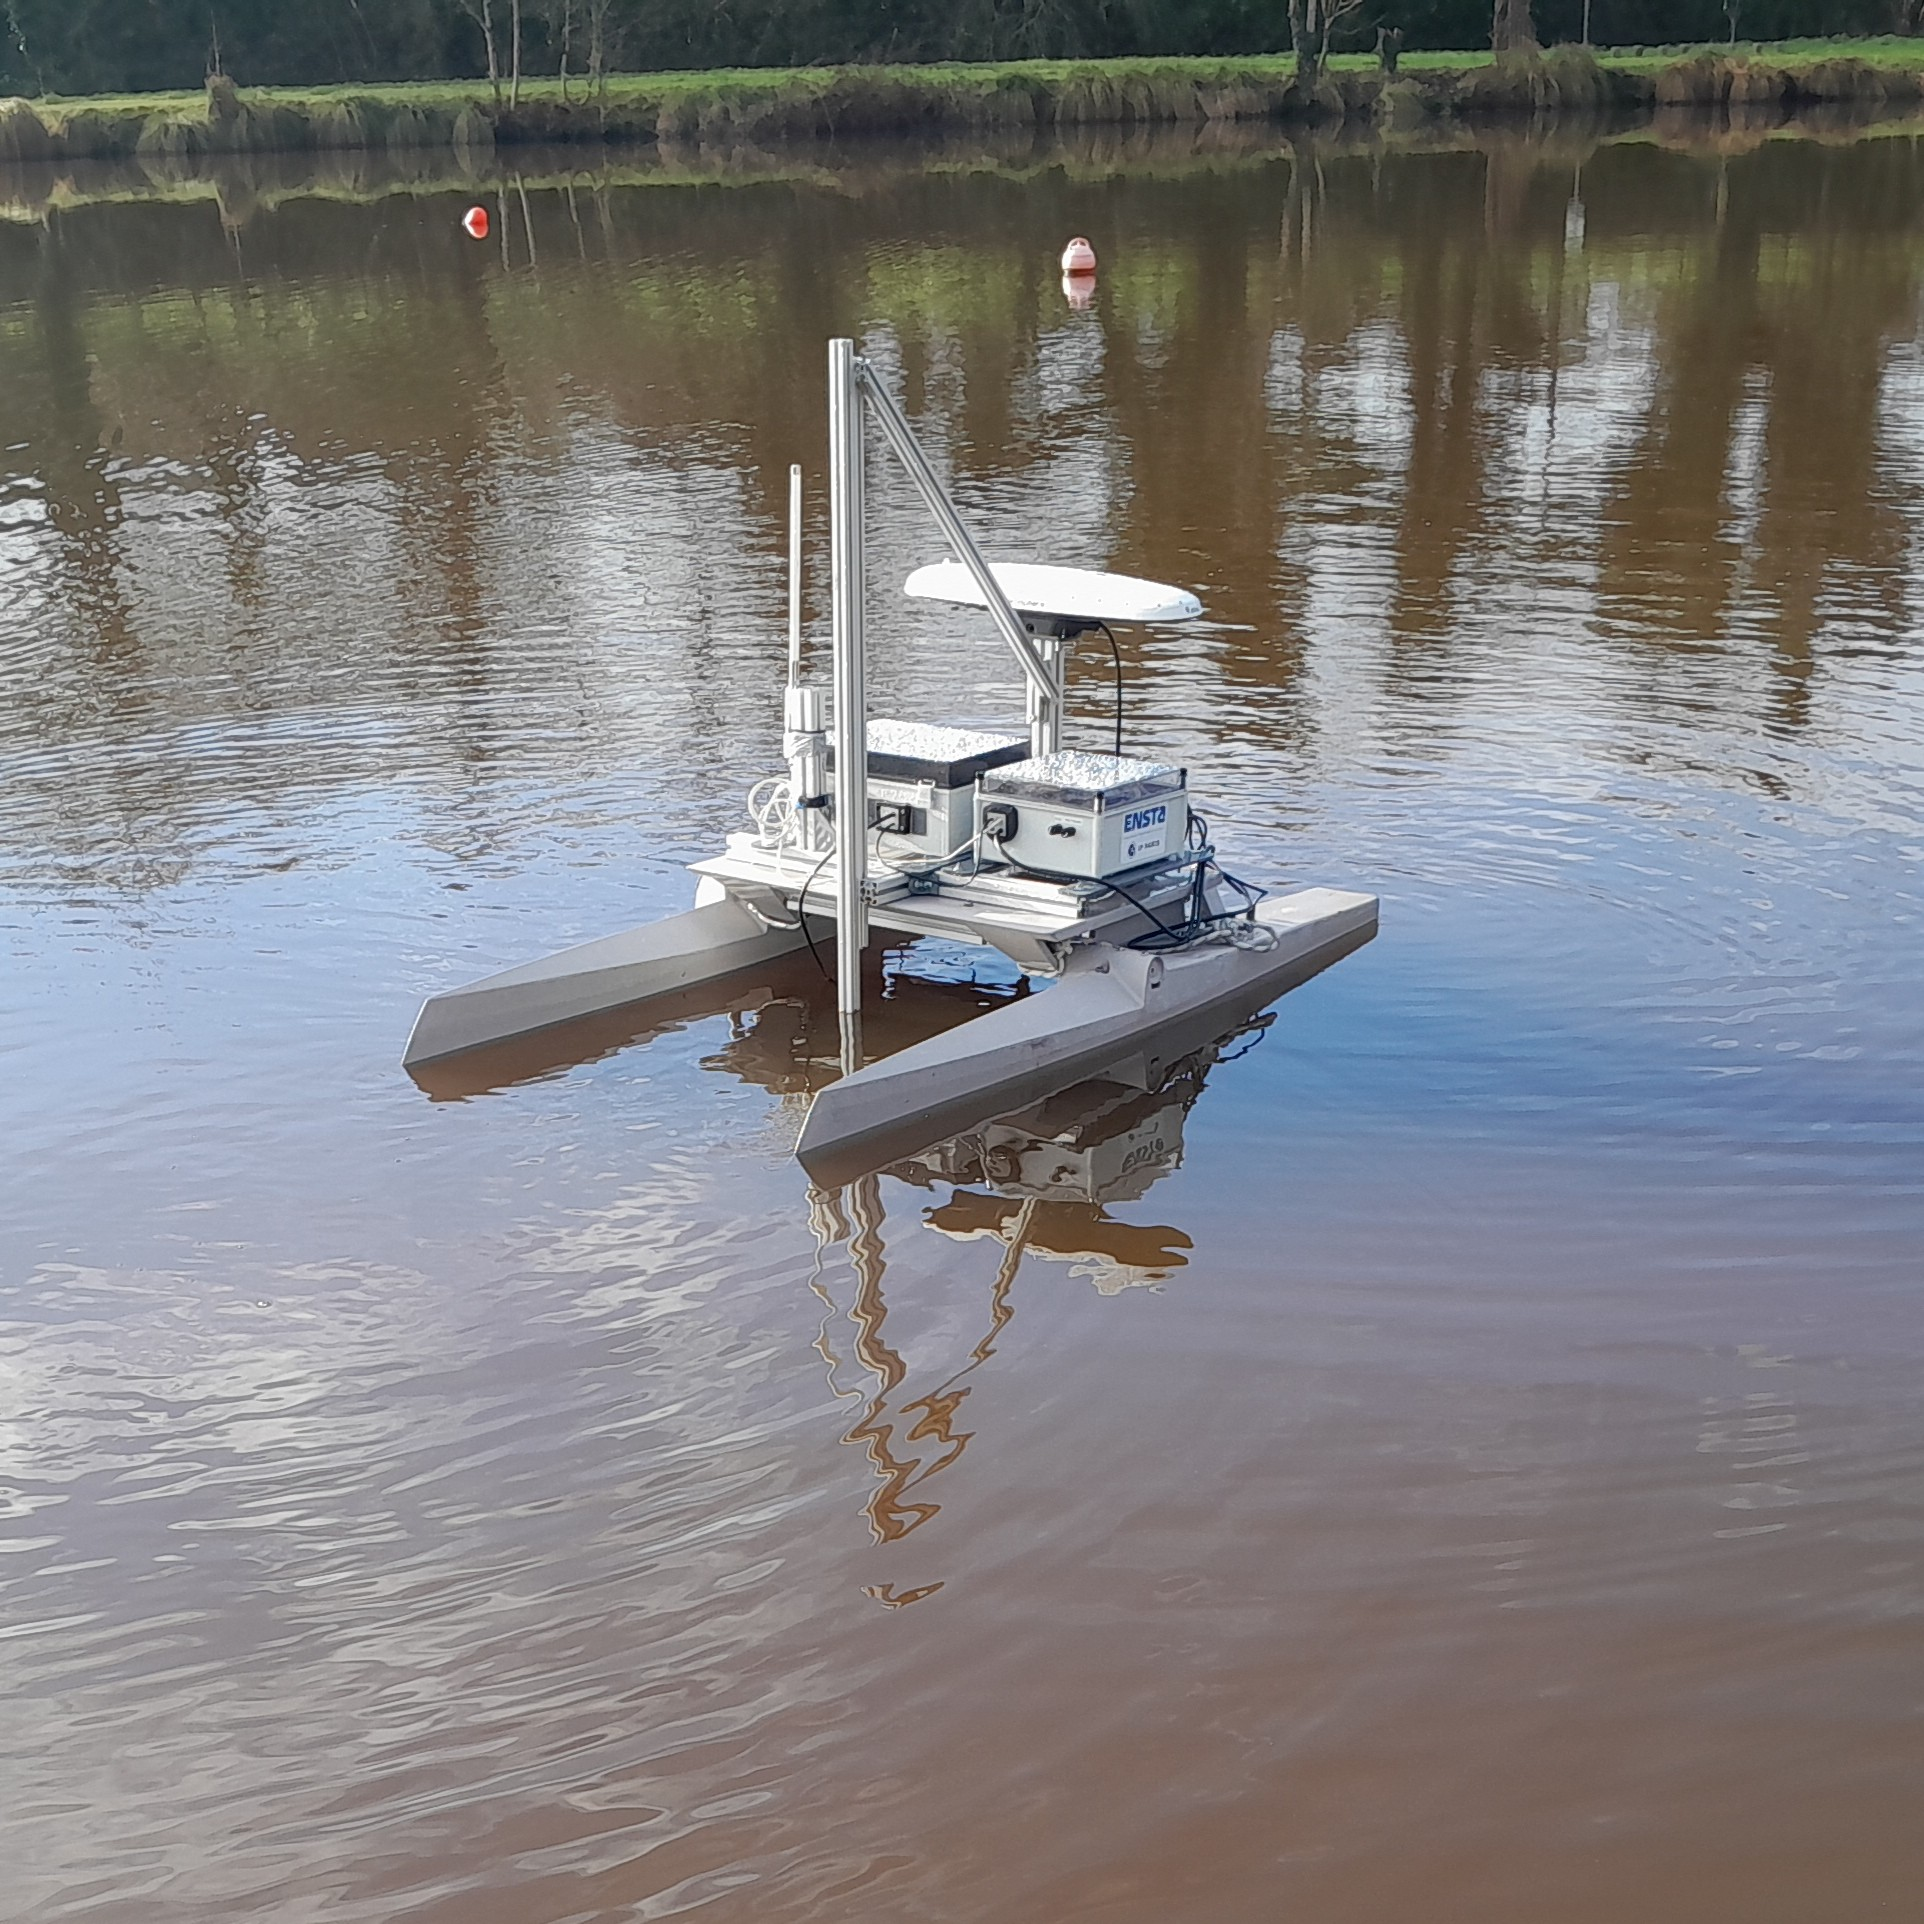
\includegraphics[width=\linewidth]{results_and_discus/figures/helios_photo.jpg}
\end{minipage}
\hfill
\begin{minipage}[t]{0.62\textwidth}
\centering
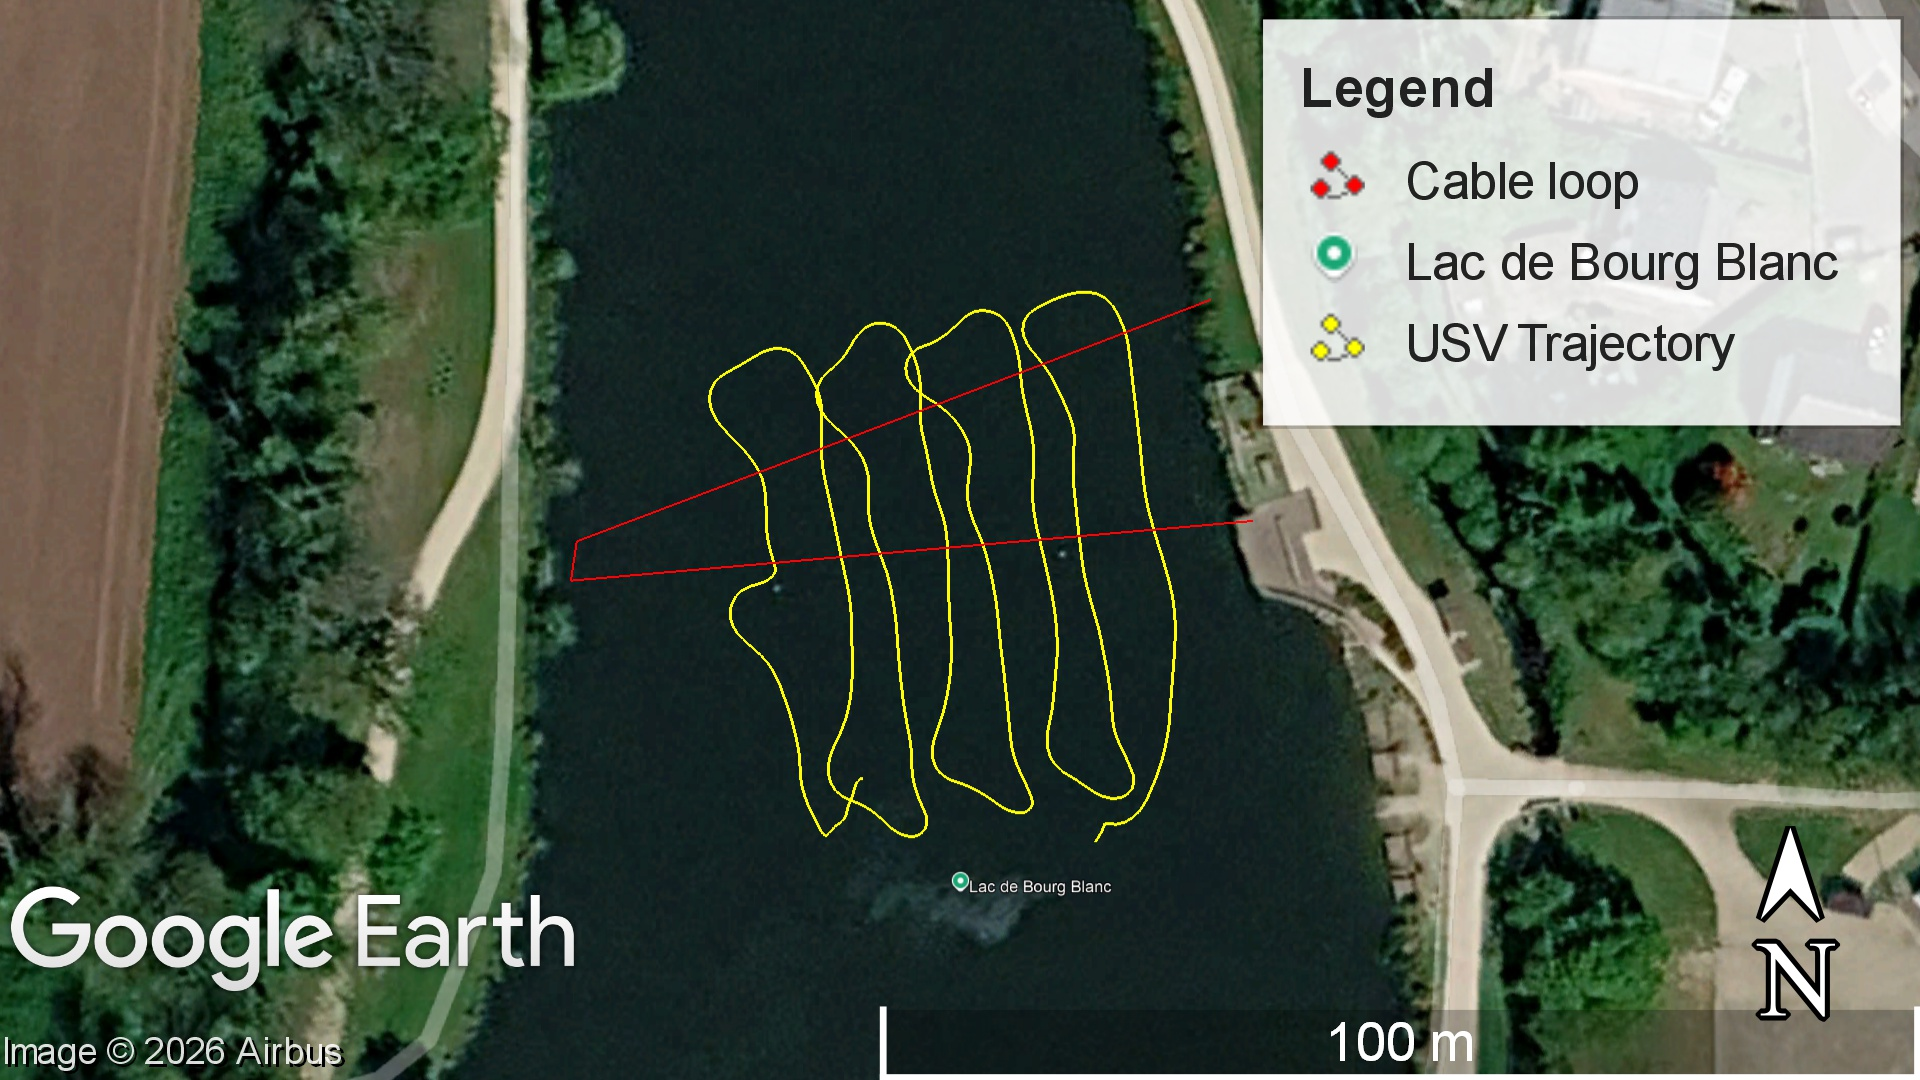
\includegraphics[width=\linewidth]{results_and_discus/figures/google_earth.jpg}
\end{minipage}
\caption{Experimental platform and test site.}
\label{fig:experiment_setup}
\end{figure*}

To set up the experiment, a loop of wire approximately 170~m long was deployed in the lake, at a depth between 1.5 and 2 meters, and energized with a DC current of 6A.
The USV was programmed to follow a lawnmower trajectory and cross the cable at a 90-degree angle with an average velocity of $0.65~m/s$.

The norm of the recorded magnetometer data was then provided as the input to the detector, as defined in Section~\ref{sec:detector}, and the filter templates—namely, the OBF—were applied over a temporal window of 32 seconds.


As a baseline, we considered MOBF of order 1 (Anderson OBF), which is the most common for dipole detection, and compared it against our cable OBF and MOBF of order 2 (dipole + quadrupole)\footnote{The order of an MOBF receiver denotes the highest multipole
retained: order~1 is the dipole (Anderson) receiver, and order~2 the
quadrupole receiver. We refer to the latter interchangeably as
``quadrupole'' (naming it by its highest retained multipole) or
``dipole~+~quadrupole'' (naming it by the source content it captures),
both designate the same order-2 receiver. These are not independent bases
stacked together, the multipolar subspaces are not in direct sum, so
order~2 is a single orthonormal set that subsumes the dipole contribution.}.

Two types of figures have been produced: first, figure \ref{fig:trajectory_comparison}, which is the drone trajectory, colored according to the measured magnetic anomaly ( $F_s - |\vec T |) $, the true cable crossing positions are marked with a star, and the detections from the filter are marked with red crosses.

A second plot, figure \ref{fig:filter_output_comparison}, represents the normalized filter input (recorded magnetic anomaly) with the normalized filter output, the crosses indicate true cable crossing moments, and the red dots represent the filter detections (which are the peaks after thresholding).


Analyzing the results, we see a clear distinction in performance: the MOBF misses the cable's exact location. In other words, the filter's maximum output lags the CPA moment by a measurable error of 1.56 and 1.9 meters for orders 1 and 2, respectively, whereas the detector based on cable OBF shows a reasonable error of 0.6 meters. 

We note that in the real experiment, part of the lag is due to localization error at the GNSS level. In Figure \ref{fig:filter_output_comparison}, we do not see isolated peaks in the filter output, and that is due to the two extremes of the cable loop being close to each other. A cleaner comparison is in the simulated experiment.


\begin{figure}[ht]
    \centering
    Cable OBF
    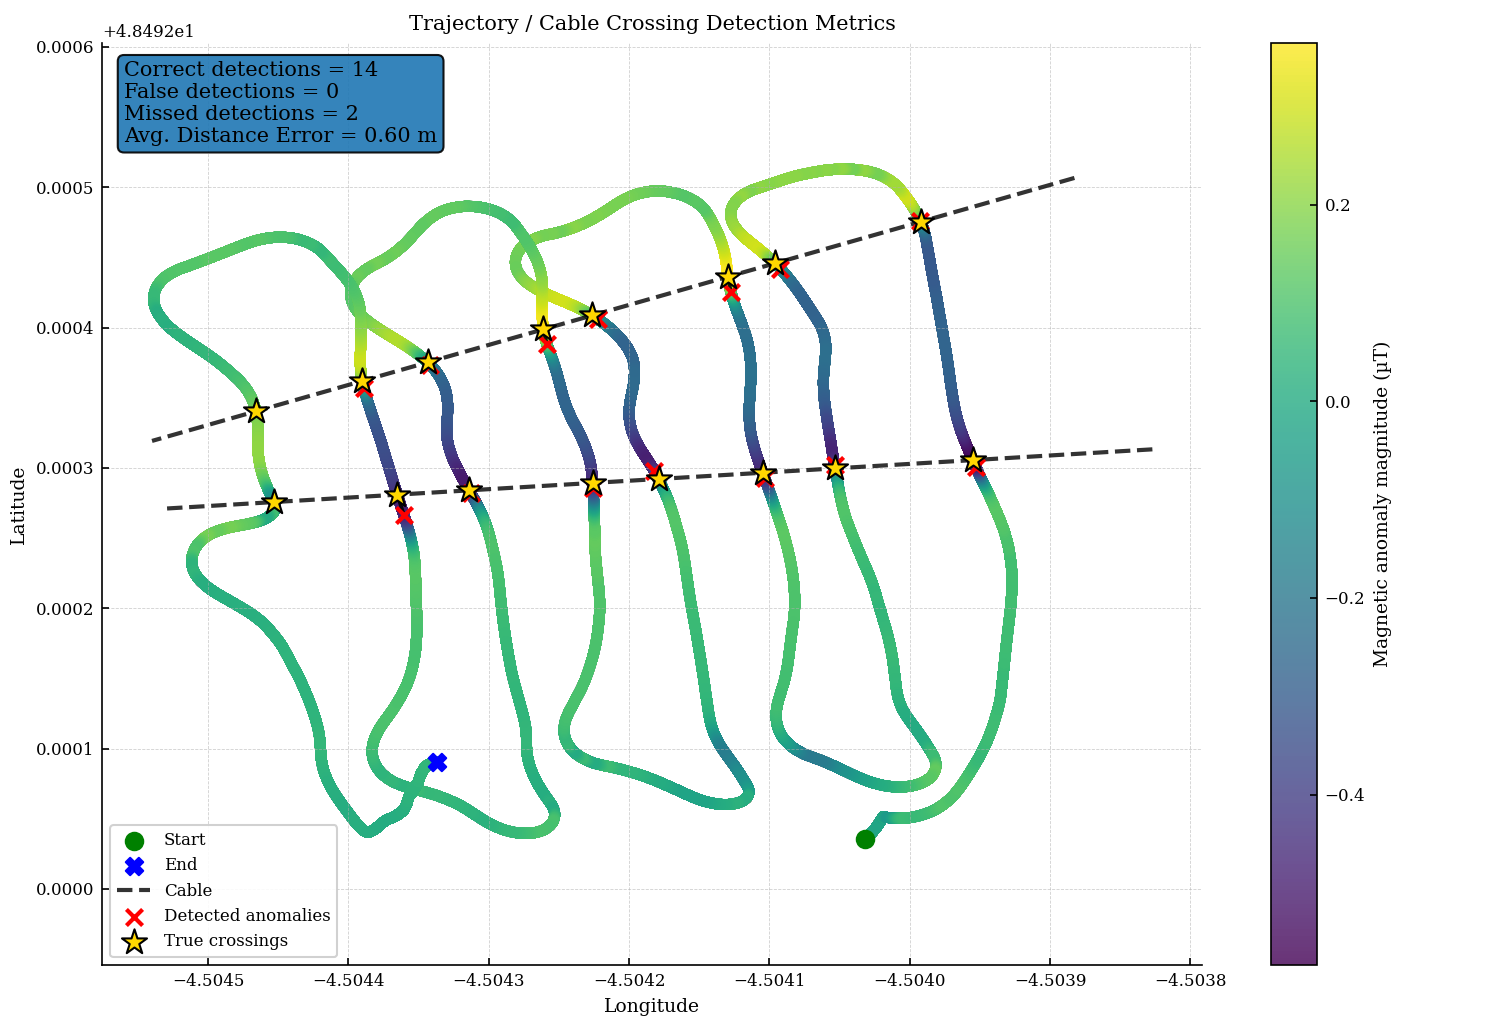
\includegraphics[width=\linewidth]{results_and_discus/figures/trajectory.png}

    MOBF order 1 (Anderson)  
    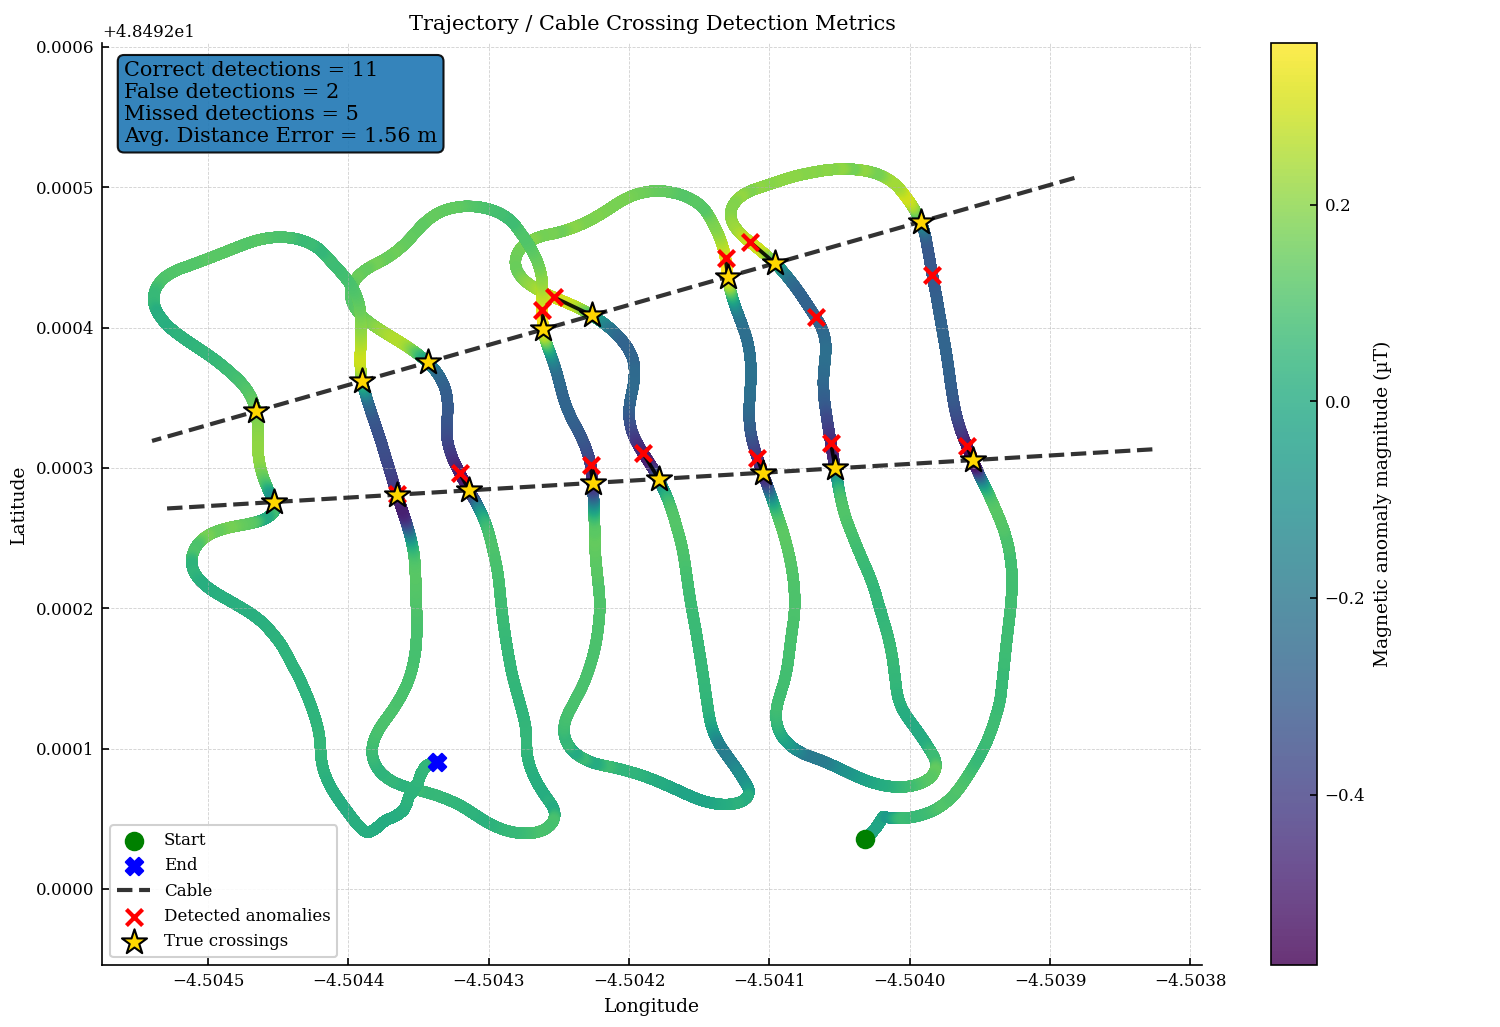
\includegraphics[width=\linewidth]{results_and_discus/figures/trajectoryAnderson.png}

    MOBF order 2 (Quadrupole)    
    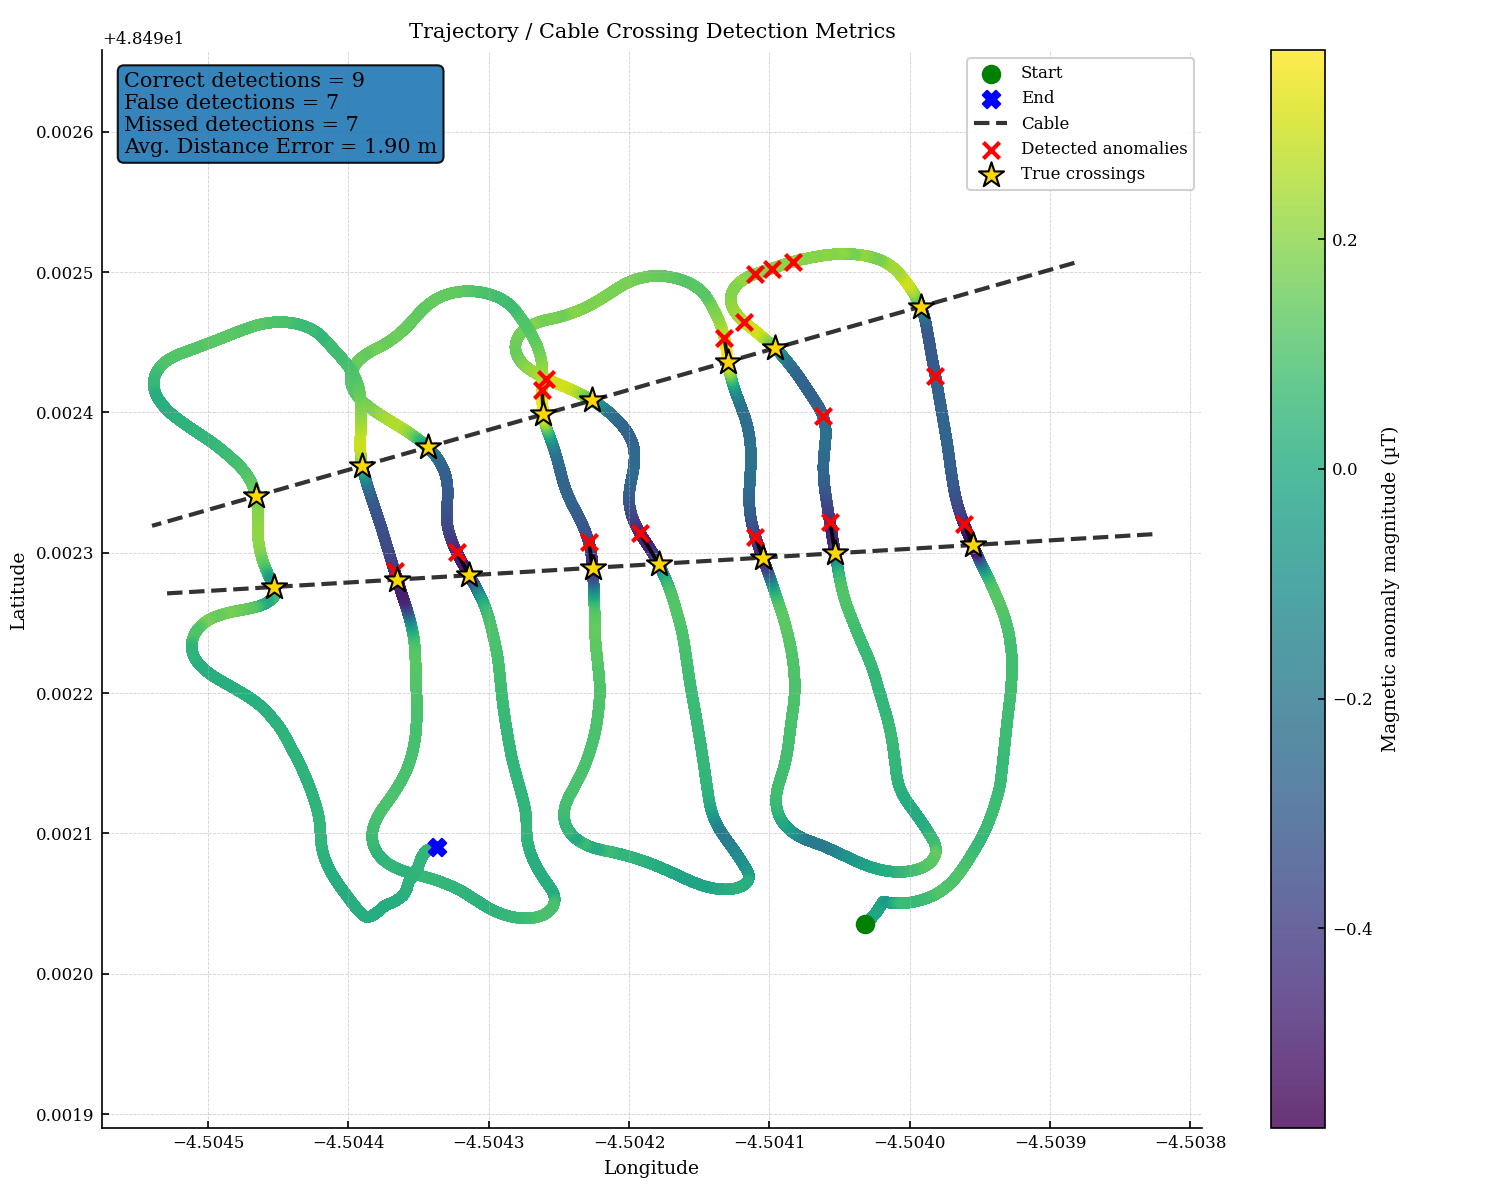
\includegraphics[width=\linewidth]{results_and_discus/figures/trajectoryQuad.png} 

    
\includegraphics[width=\linewidth]{results_and_discus/figures/trajectory_legends.png}
    \caption{Comparison of detection locations along the USV trajectory relative to the cable position. The color indicates the data entering the filter. Top: detections using the cable OBF. Middle: detections using the dipole OBF. Bottom: detections using the quadrupole MOBF.}
    \label{fig:trajectory_comparison}
\end{figure}

\begin{figure}[ht]
    \centering
    Cable OBF    
    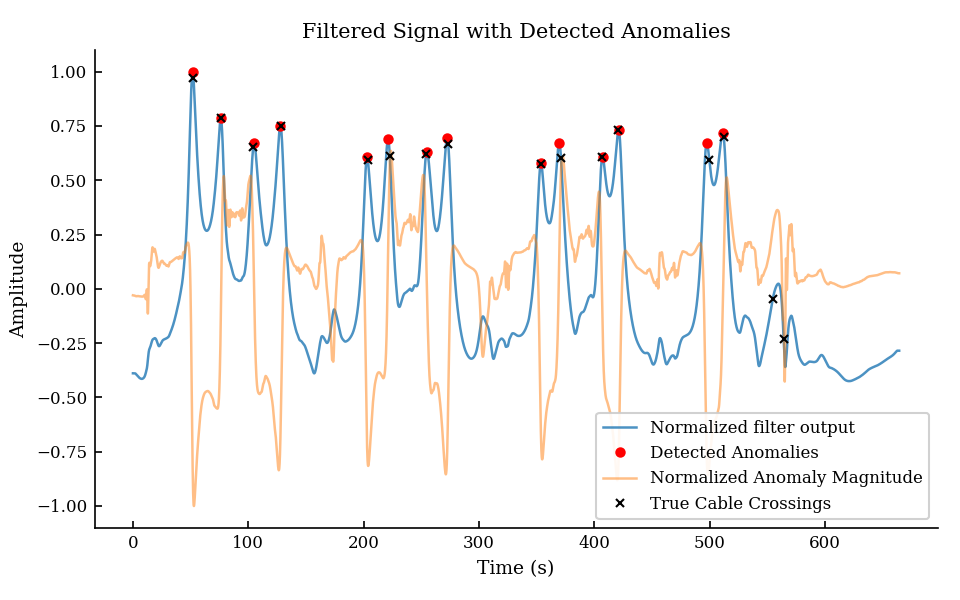
\includegraphics[width=\linewidth]{results_and_discus/figures/filter_output.png}

    
    MOBF order 1 (Anderson)
    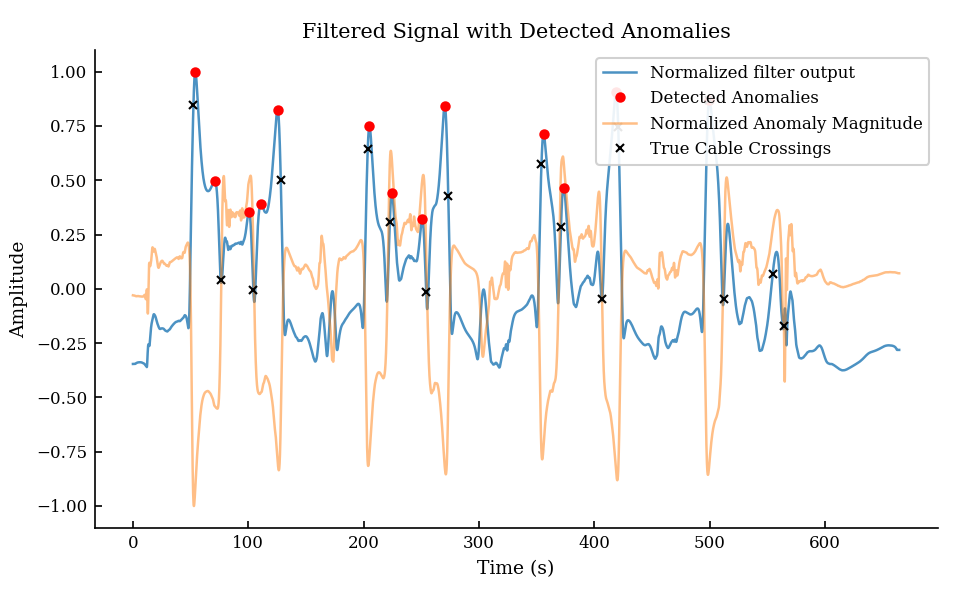
\includegraphics[width=\linewidth]{results_and_discus/figures/filter_outputAnderson.png}
    
    MOBF order 2 (Quadrupole)
    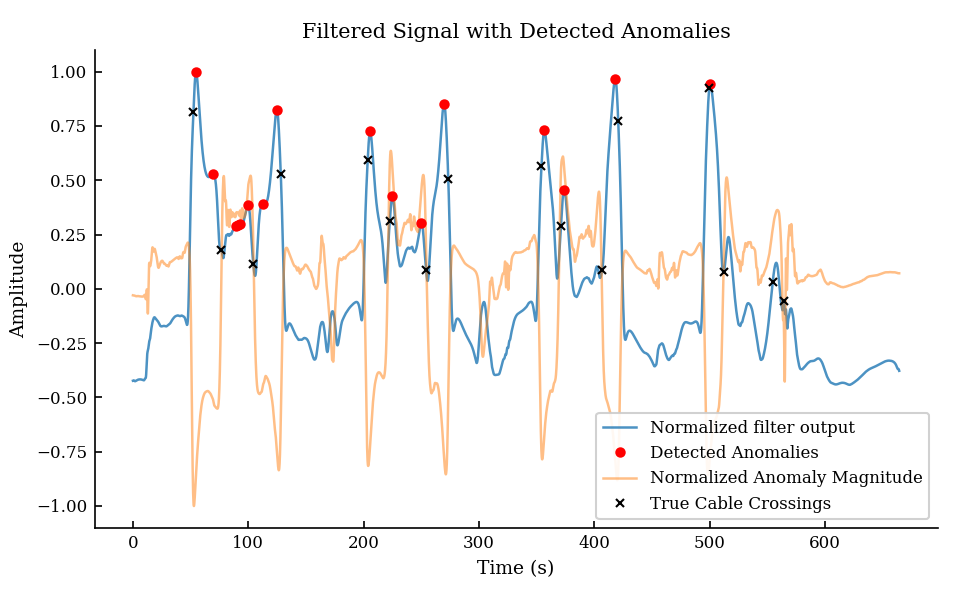
\includegraphics[width=\linewidth]{results_and_discus/figures/filter_outputQuad.png}
    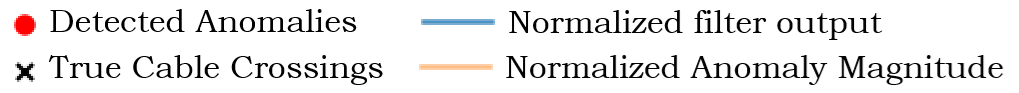
\includegraphics[width=\linewidth]{results_and_discus/figures/filter_output_legends.png}
    \caption{Comparison of filter outputs with detections and true cable crossings. 
    Top: output using the cable OBF. Middle: output using the dipole OBF. Bottom: output using the quadrupole MOBF.}
    \label{fig:filter_output_comparison}
\end{figure}

\subsubsection{Simulation}\label{sec:simulation}

We developed a Python-based simulation framework that produces synthetic trajectories of GNSS coordinates and the corresponding recorded magnetic field for controlled sensor configurations and experimental setups.

Here we simulated the magnetic field of an electric wire following the Biot-Savart law, see equation \ref{eq:mag_field}, and as a trajectory we took a lawnmower pattern with constant velocity $v=1.8~m/s$, the cable depth goes from 1 to 1.5 meters, linearly from start to finish. It carries a DC current of 6A, and the results were mixed with AWGN so that we obtained an SNR of -6dB
\footnote{signal to noise ratio $
\mathrm{SNR}_{\mathrm{dB}}
=
10 \log_{10}\left(
\frac{\sum_t X(t)^2}{\sigma^2}
\right).
$ with $X(t)$ the norm of the recorded magnetic field, and $\sigma^2$ the variance of an AWGN.}.
The simulation was executed at a sampling frequency of 50 Hz, and the same analysis parameters and graphical representations employed in the real experiment were applied here, as illustrated in \autoref{fig:trajectory_comparison_simu}.

Analyzing the plots, we see a similar behavior to that of the real experiment, as our cable OBF, detected the cable presence at the exact moment with so little error (average error of 0.09~meters). The same could not be said for MOBF, as its first order (Anderson), detected the cable with a noticeable lag, leading to a constant localization error of 1.47~meters. A minor observation is that the amplitude exhibits two maxima per crossing. This behavior is most clearly evidenced by the smaller secondary peak around 50~s in Figure \ref{fig:filter_output_comparison_simu} (middle).

In the simulations, the SNR was lower than in the corresponding physical experiments. Under these conditions, the second-order MOBF produced output with increased noise levels and less well-defined peaks, thereby degrading the accuracy and robustness of the localization, giving a better average distance error than the first order (only 0.65~meters), but it is much noisier.

These findings empirically support the superior performance of cable OBF for this study, given that precise and reliable localization constitutes the primary objective of the project.


\begin{figure}[ht]
    \centering
    Cable OBF
    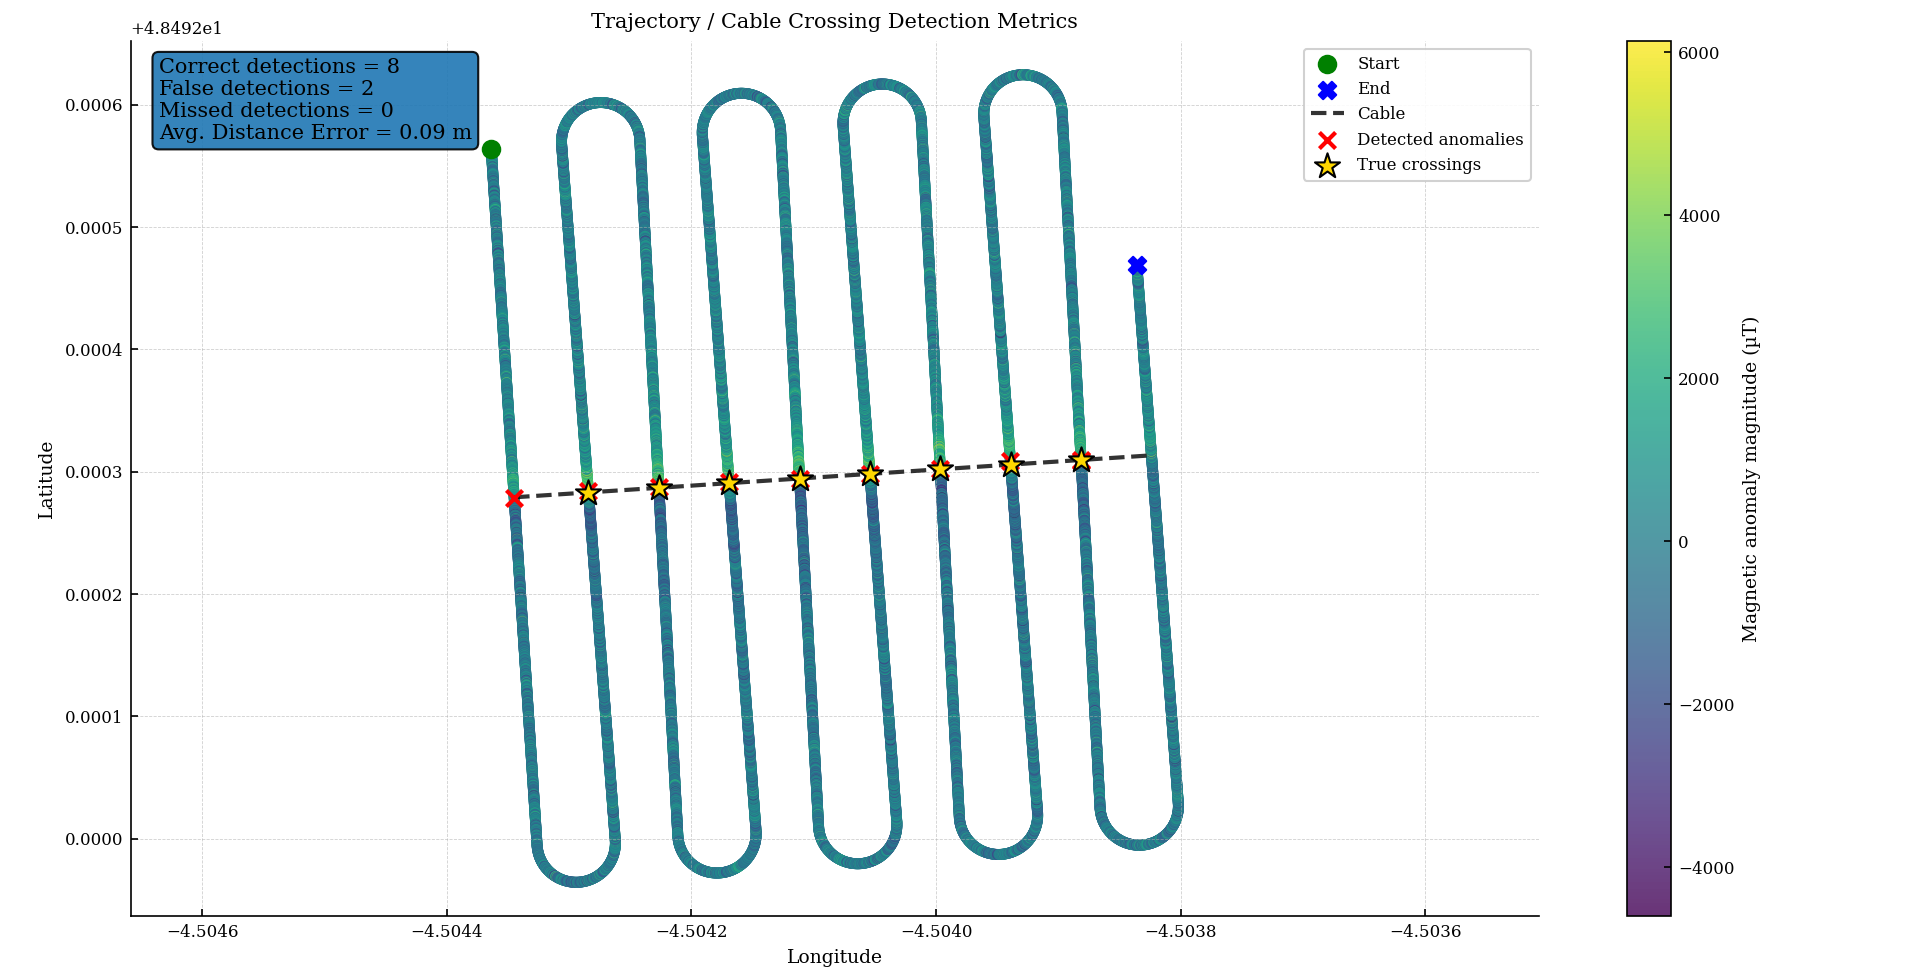
\includegraphics[width=\linewidth]{results_and_discus/figures/trajectory_simu_noisy.png}
    
    MOBF order 1 (Anderson)
    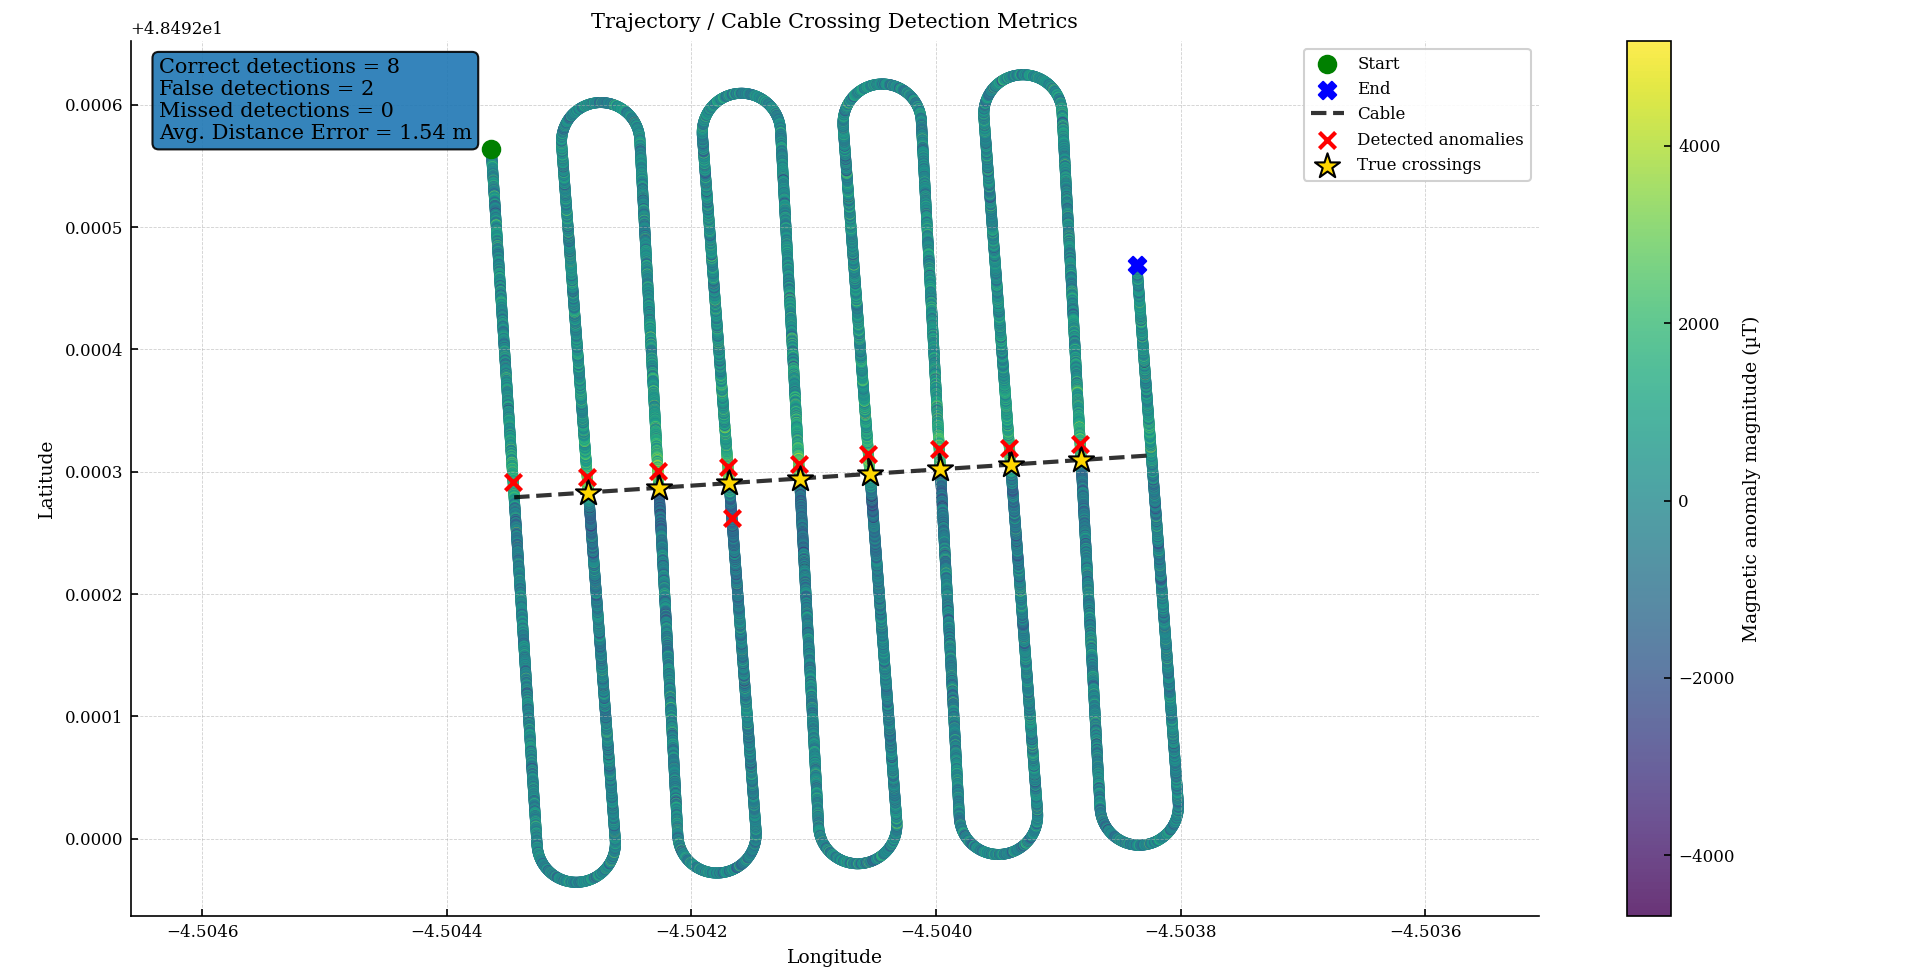
\includegraphics[width=\linewidth]{results_and_discus/figures/trajectoryAnderson_simu_noisy.png}
    
    MOBF order 2 (Quadrupole)
    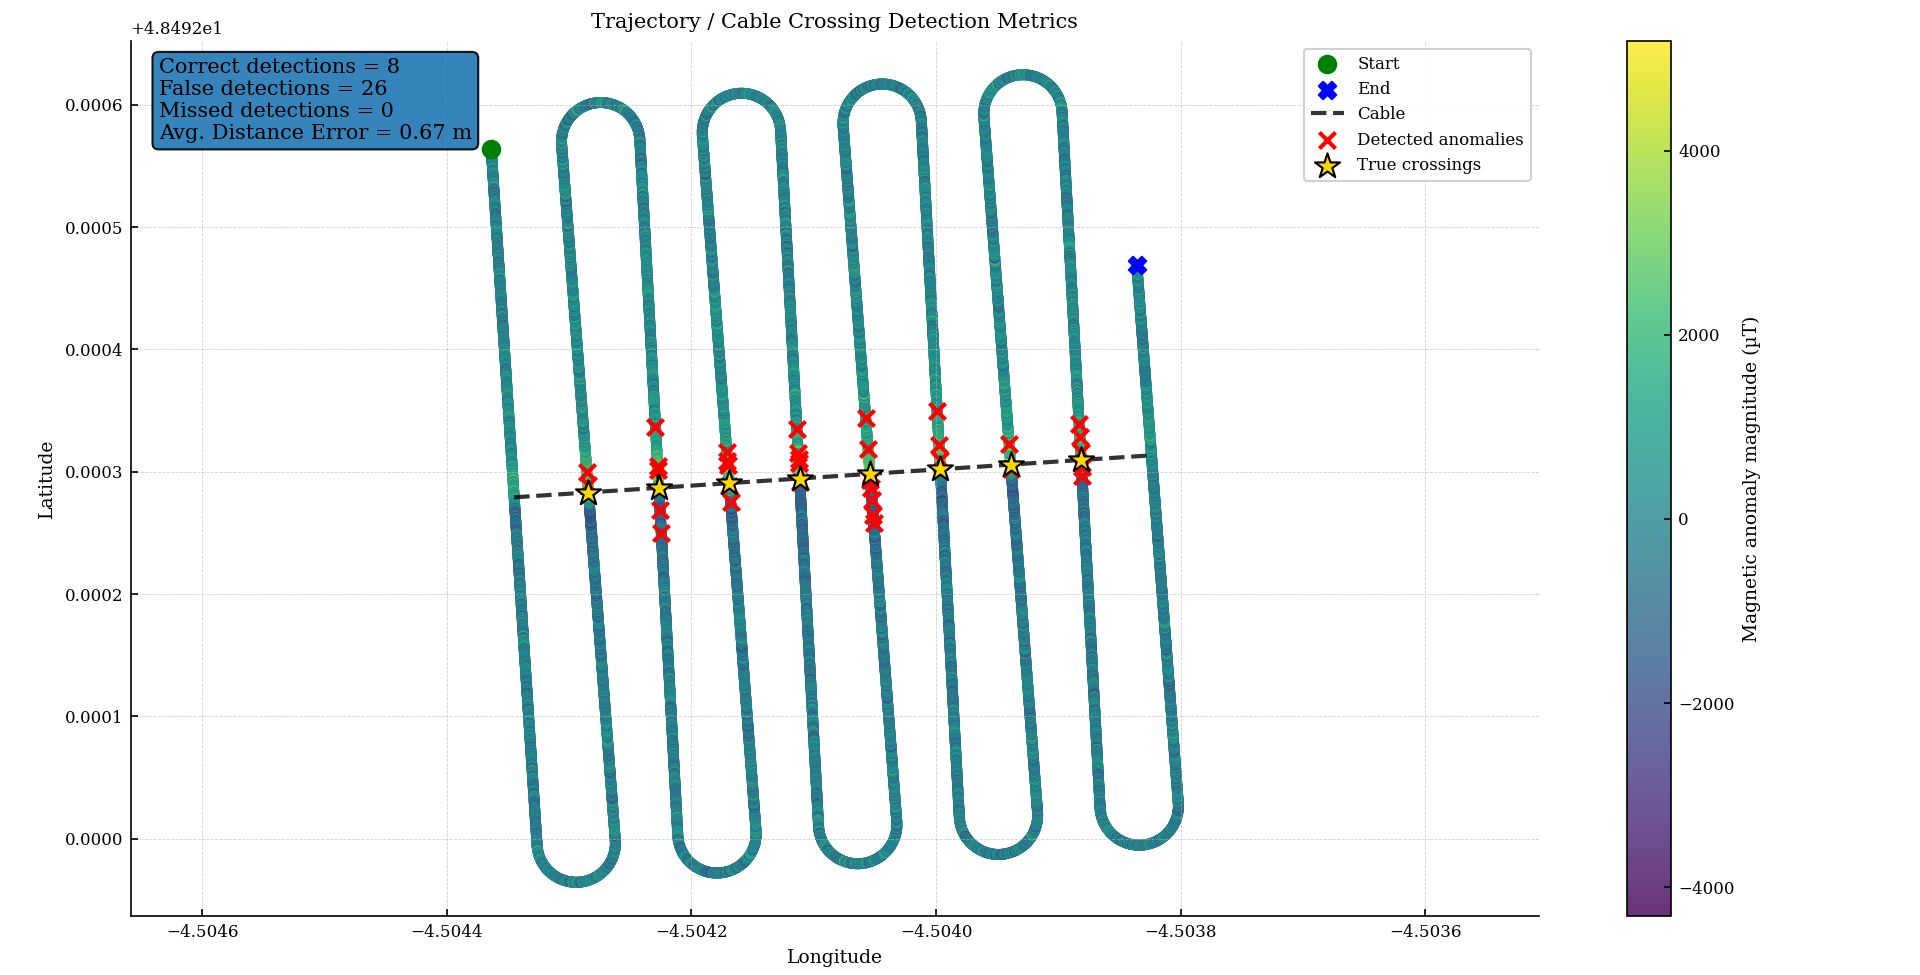
\includegraphics[width=\linewidth]{results_and_discus/figures/trajectoryquad_simu_noisy.png} 
    
\includegraphics[width=\linewidth]{results_and_discus/figures/trajectory_legends.png}
    \caption{Comparison of detection locations along the USV trajectory relative to the cable position. The color indicates the data entering the filter. Top: detections using the cable OBF. Middle: detections using the dipole OBF. Bottom: detections using the quadrupole MOBF.}
    \label{fig:trajectory_comparison_simu}
\end{figure}


\subsection{Comparison with the Multipolar Framework}

In complement to the experimental and simulation results, this subsection examines the detection performance and associated energy capture properties.

In the MOBF study \cite{chenevas2025multipolar}, it was demonstrated that a matched receiver is not necessarily the optimal detector. For a multipolar source, projecting the data onto a lower-order subspace can yield superior detection performance, because such a subspace captures most of the signal energy while involving fewer noise-dominated dimensions. In other words, there is a trade-off between capturing more signal energy by increasing the order of the subspace and reducing the noise contribution by restricting attention to a lower-order subspace.

The two experiments presented below demonstrate that this effect cannot occur in our setting, for a structural reason: the cable does not behave as a multipole of any finite order, since its field decays too slowly. Consequently, in our comparison the lower-dimensional receiver coincides with the matched receiver, which simultaneously provides full signal energy capture and the minimal possible dimensionality.

In both the MOBF framework and the present work, the detectors are structurally very similar; the only difference lies in the choice of templates. Specifically, we define the test statistic
\begin{equation}
    T = \sum_{p=1}^{P} \langle x, g_p \rangle^2,
\end{equation}
where $T$ denotes the filter output, $P$ is the number of orthonormal basis functions, and $g_p$ denotes one of the OBF.

\subsubsection{experiment 1, energy capture vs. MOBF order}
we take the cable's clean along the trak anomaly $s$, see equation \ref{eq:anomaly}. for each multipolar order M=1 (dipole/Anderson),2(Quadripole), 3 (octopole), we built the MOBF (see table \ref{tab:basis_comparison}) and computed the fraction of $s$'s energy that lives in that subspace spanned by the MOBF.
\begin{equation}
    \eta (M) = \frac{T^2}{||s||^2}
\end{equation}

for s we took arbitrarily realistic parameters ($v=1.8 \ m/s; \ d=1\ m; \ \theta =90^\circ;\ \psi=45^\circ;\ \delta=60^\circ$); to calculate $\eta$ table \ref{tab:energy_capture}
\begin{table}[ht]
\centering

\resizebox{\columnwidth}{!}{%
\begin{tabular}{|c|c|c|c|c|}
\hline
\textbf{Basis} &
\shortstack{\textbf{Cable OBF}} &
\shortstack{\textbf{Dipole}\\$(M=1)$} &
\shortstack{\textbf{Quadrupole}\\$(M=2)$} &
\shortstack{\textbf{Octupole}\\$(M=3)$} \\
\hline
$\eta$ & 1.000 & 0.495 & 0.657 & 0.750 \\
\hline
\end{tabular}%
}
\caption{Energy capture of the cable signal by each receiver.}
\label{tab:energy_capture}
\end{table}

$\eta_{cable} = 1$ for our cable OBF, by construction.

The results show that $\eta(M) < 1$for every finite, numerically usable M, and raising M helps only marginally (the basis functions decay ever faster, beyond M=3, rendering them unusable \cite{chenevas2025multipolar}).

\subsubsection{ROC and SNR}

Building on the previous results, we evaluated the receiver operating characteristic (ROC) curve using both the analytical expression reported in \cite{Kay1998Detection},
\[
P_d = \bar F_{\chi^2_v(\lambda)}\bigl(\bar F_{\chi^2_v}^{-1}(P_{fa})\bigr),
\]
and a Monte Carlo simulation with \(2\times 10^4\) realizations, Figure~\ref{fig:ROCvsSNR}. For each SNR value, we computed the area under the curve (AUC), Figure~\ref{fig:AUCvsSNR}.

\begin{figure*}
    \centering
    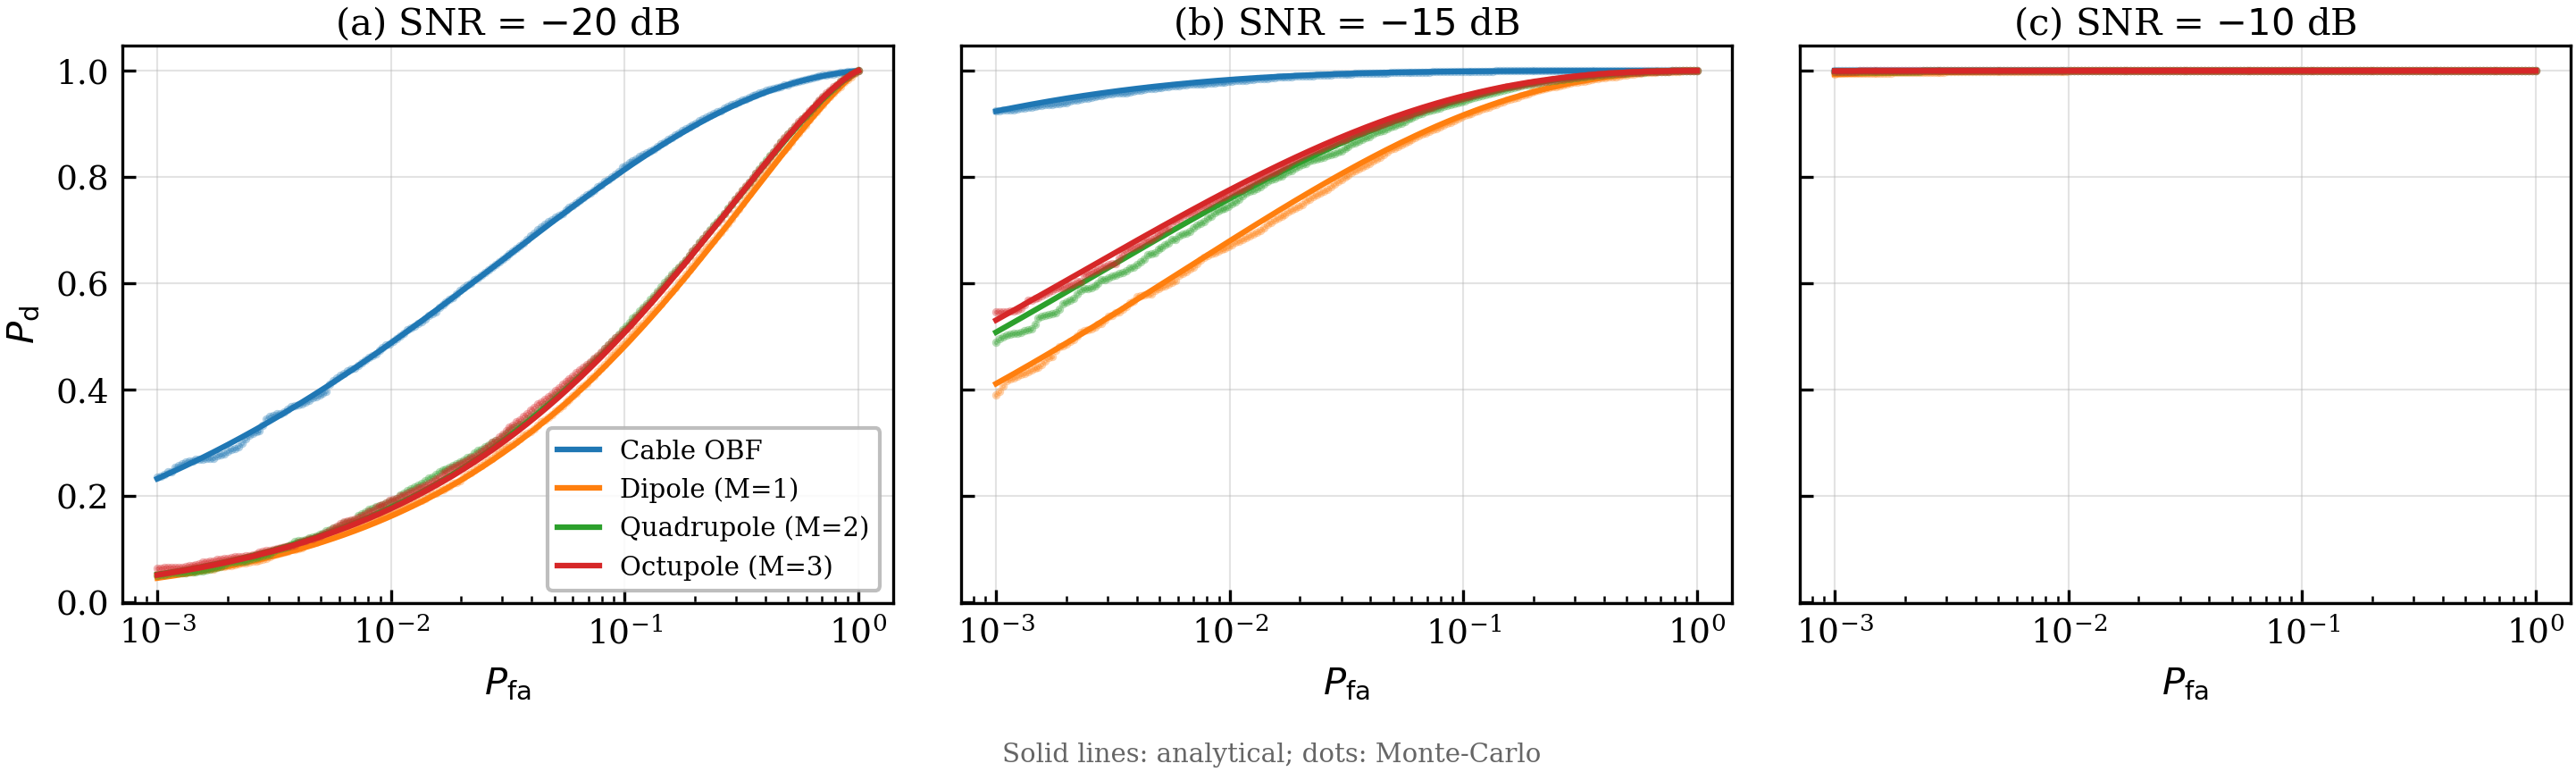
\includegraphics[width=1\textwidth]{results_and_discus/figures/ROCvsSNR.png}
    \caption{ROC curves for the cable OBF and MOBF receivers at several SNR levels obtained from the analytical form and by Monte Carlo simulation ($2\times10^4$ realizations).}
    \label{fig:ROCvsSNR}
\end{figure*}

\begin{figure}
    \centering
    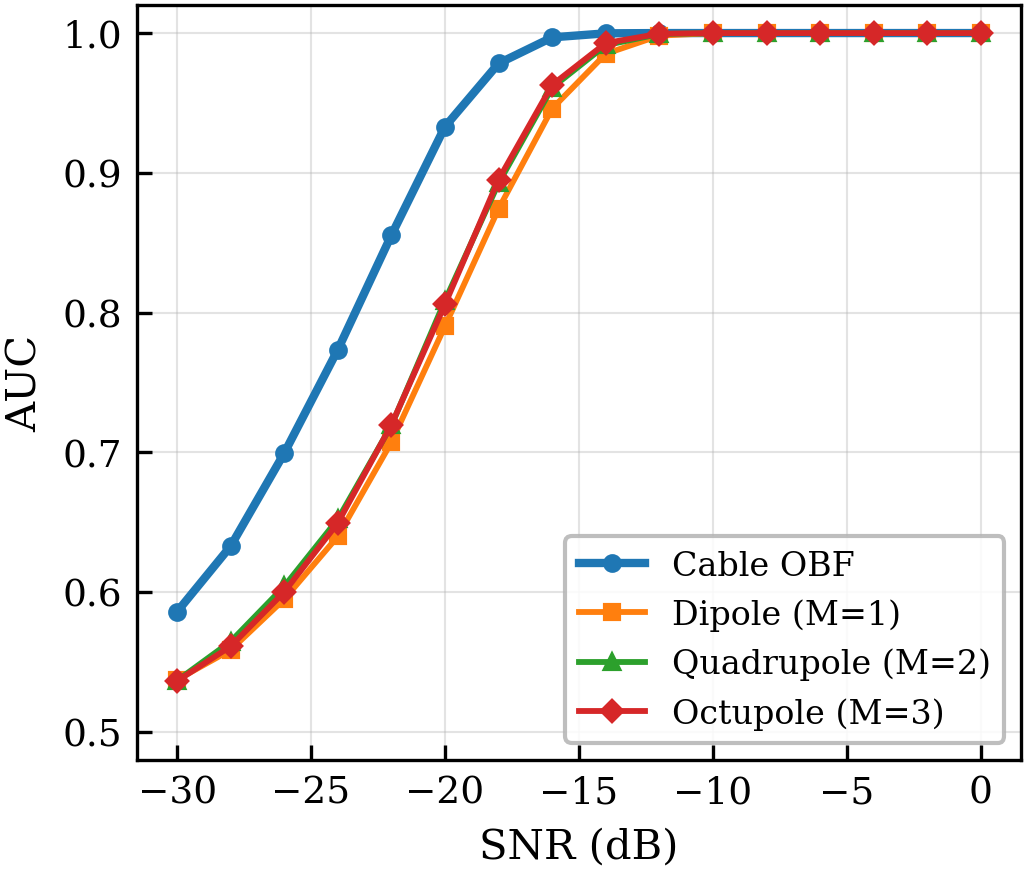
\includegraphics[width=\linewidth]{results_and_discus/figures/AUCvsSNR.png}
    \caption{Area under the ROC curve (AUC) as a function of SNR for the cable OBF and MOBF receivers of orders 1 to 3.}
    \label{fig:AUCvsSNR}
\end{figure}

Disregarding the detection offset discussed in section~\ref{sec:simulation}, the results here indicate that the MOBF is capable of detecting the cable. However, they also show that the matched cable OBF consistently outperforms or matched all considered MOBF orders, with the performance gap becoming particularly pronounced at SNR values below \(-15\)~dB. This behavior is attributable to the fact that the cable OBF captures the full energy of the signal \(s\) while involving the minimum number of noisy channels.

Finally, the behavior observed in Figure~\ref{fig:AUCvsSNR} is reproduced in Figure~\ref{fig:paramJumble} for different combinations of \(\psi\) and \(\delta\), providing further evidence that the cable OBF outperforms the MOBF for cable detection.


\begin{figure}
    \centering
    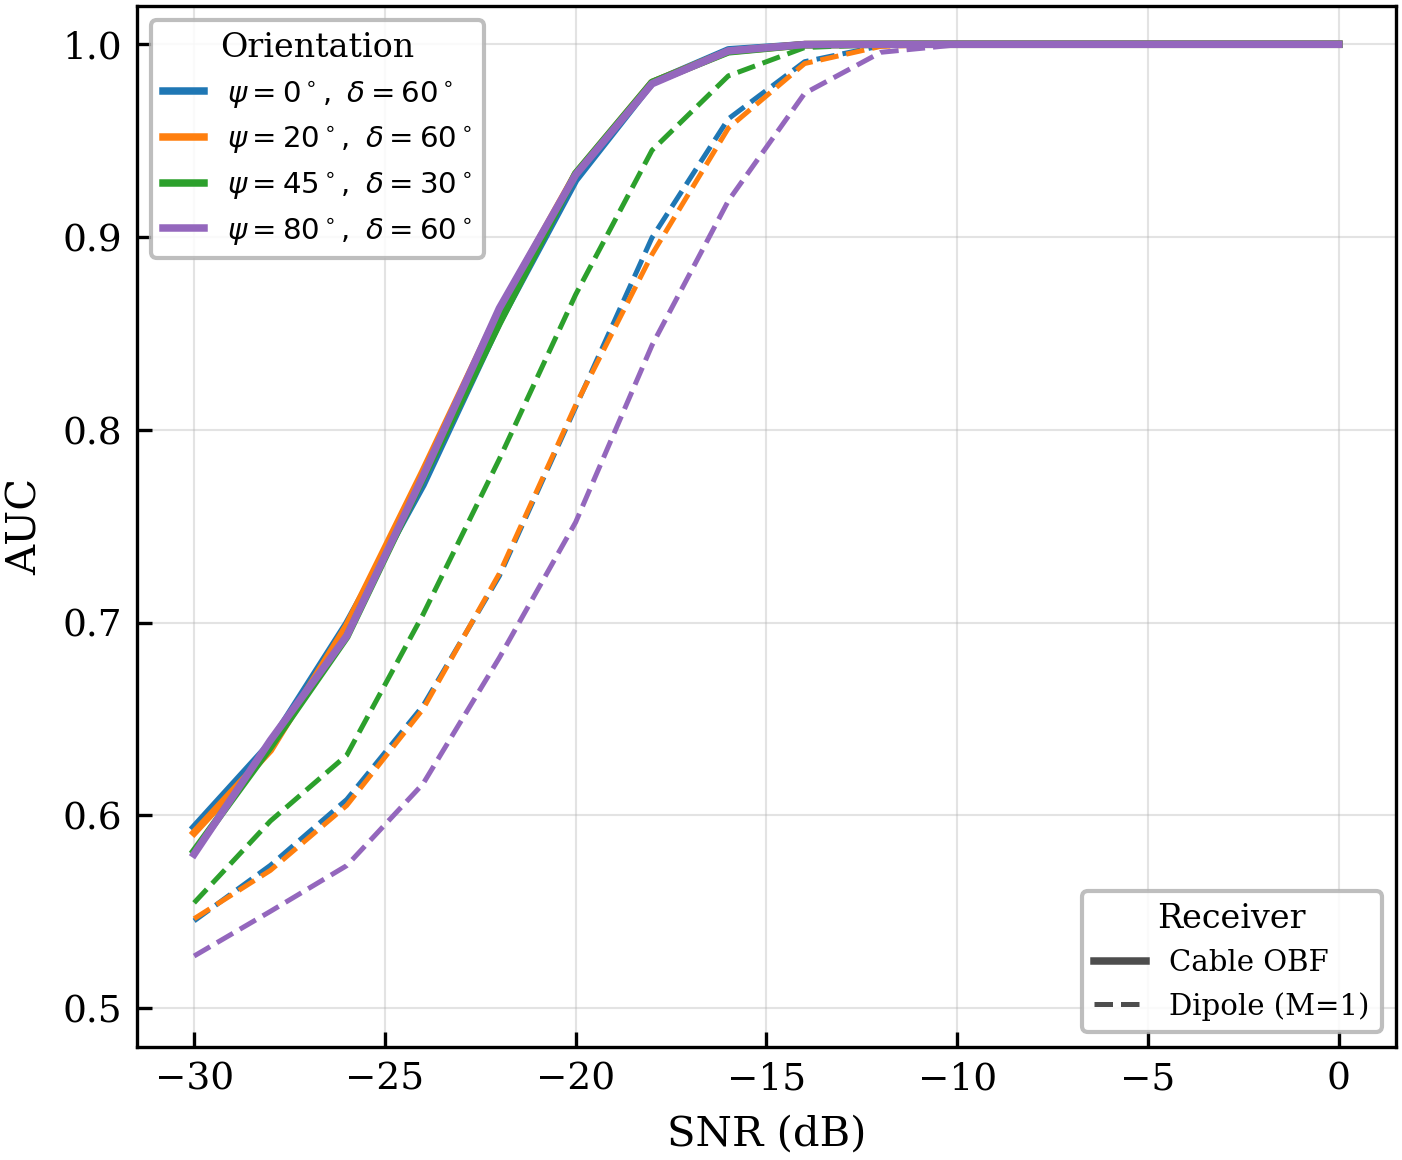
\includegraphics[width=\linewidth]{results_and_discus/figures/params_jumble.png}
    \caption{AUC as a function of SNR for varying orientation parameters $\psi$ and $\delta$ confirming that the cable OBF consistently outperforms MOBF receivers across orientations.}
    \label{fig:paramJumble}
\end{figure}
\subsection{Structural and Physical Analysis}\label{sec:SnP}

\highlight{\begin{table}[ht!]
\centering
\renewcommand{\arraystretch}{2.5}
\begin{tabular}{|c|c|c|}
\hline
\textbf{Source} & \textbf{Basis $g_p(\tau)$} & \textbf{Function} \\
\hline
\multirow{2}{*}{Cable}
    & $\Phi_1(\tau)$ (even)
    & $\displaystyle\sqrt{\frac{2}{\pi}}\,\frac{1}{1+\tau^2}$\\
    & $\Phi_2(\tau)$ (odd)
    & $\displaystyle\sqrt{\frac{2}{\pi}}\,\frac{\tau}{1+\tau^2}$\\
\hline
\multirow{3}{*}{Dipole (Anderson)}
    & $g_{1,1}(\tau)$ (even)
    & $\displaystyle\frac{\sqrt{128/35\pi}}{(1+\tau^2)^{5/2}}$\\
    & $g_{1,2}(\tau)$ (odd)
    & $\displaystyle\frac{\sqrt{128/5\pi}\;\tau}{(1+\tau^2)^{5/2}}$\\
    & $g_{1,3}(\tau)$ (even)
    & $\displaystyle\frac{\sqrt{56/\pi}\;(\tau^2-1/7)}{(1+\tau^2)^{5/2}}$\\
\hline
\multirow{5}{*}{Quadrupole}
    & $g_{2,1}(\tau)$ (even)
    & $\displaystyle\frac{32}{\sqrt{231\pi}\,(1+\tau^2)^{7/2}}$\\
    & $g_{2,2}(\tau)$ (odd)
    & $\displaystyle\frac{-32\,\tau}{\sqrt{21\pi}\,(1+\tau^2)^{7/2}}$\\
    & $g_{2,3}(\tau)$ (even)
    & $\displaystyle\frac{8\sqrt{154}\,(11\tau^2-1)}{77\sqrt{\pi}\,(1+\tau^2)^{7/2}}$\\
    & $g_{2,4}(\tau)$ (odd)
    & $\displaystyle\frac{8\sqrt{6}\,\tau\,(1-3\tau^2)}{3\sqrt{\pi}\,(1+\tau^2)^{7/2}}$\\
    & $g_{2,5}(\tau)$ (even)
    & $\displaystyle\frac{4\sqrt{21}\,(21\tau^4-18\tau^2+1)}{21\sqrt{\pi}\,(1+\tau^2)^{7/2}}$\\
\hline
\end{tabular}
\caption{Comparison of cable, dipole (Anderson), and quadrupole orthonormal basis functions (obtained using the Gegenbauer polynomials formulation from \cite{chenevas2025multipolar}).} 
\label{tab:basis_comparison}
\end{table}
Returning to the statement made in the introduction, MOBFs are designed to represent spatially bounded (compact) sources enclosed within a finite Brillouin sphere. This configuration is fundamentally different from the infinite cable geometry, for which the source effectively extends without bound. In particular, the observation point can never lie outside the Brillouin sphere that encloses the source, and the inability of the MOBF expansion to reproduce the cable’s decay rate is a direct manifestation of this geometric incompatibility.

This discrepancy is readily seen from the analytical expressions in Table~\ref{tab:basis_comparison}. For the cable OBF, the slowest decay rate is of order -1, as exhibited by the function $\phi_2(\tau)$. By contrast, an MOBF of order $M$ belongs to the space
$
\operatorname{span}\!\left\{\frac{\tau^n}{(1+\tau^2)^{M+3/2}}\right\}_{n=0}^{2M},
$
for which the slowest decay rate is given by $2M - 2\left(M+\tfrac{3}{2}\right) = -3$. This decay rate is independent of the multipole order $M$ and is strictly faster than the slowest cable decay rate of $-1$, so no finite multipole order can match the cable's behavior. Consequently, there is no multipole order whose decay matches that of the cable: every multipole decays more rapidly. As a result, any finite truncation of the multipole expansion necessarily fails to capture the full contribution of the field in the far tails.}


\begin{figure}[ht]
\centering

\begin{minipage}{0.75\linewidth}
\centering
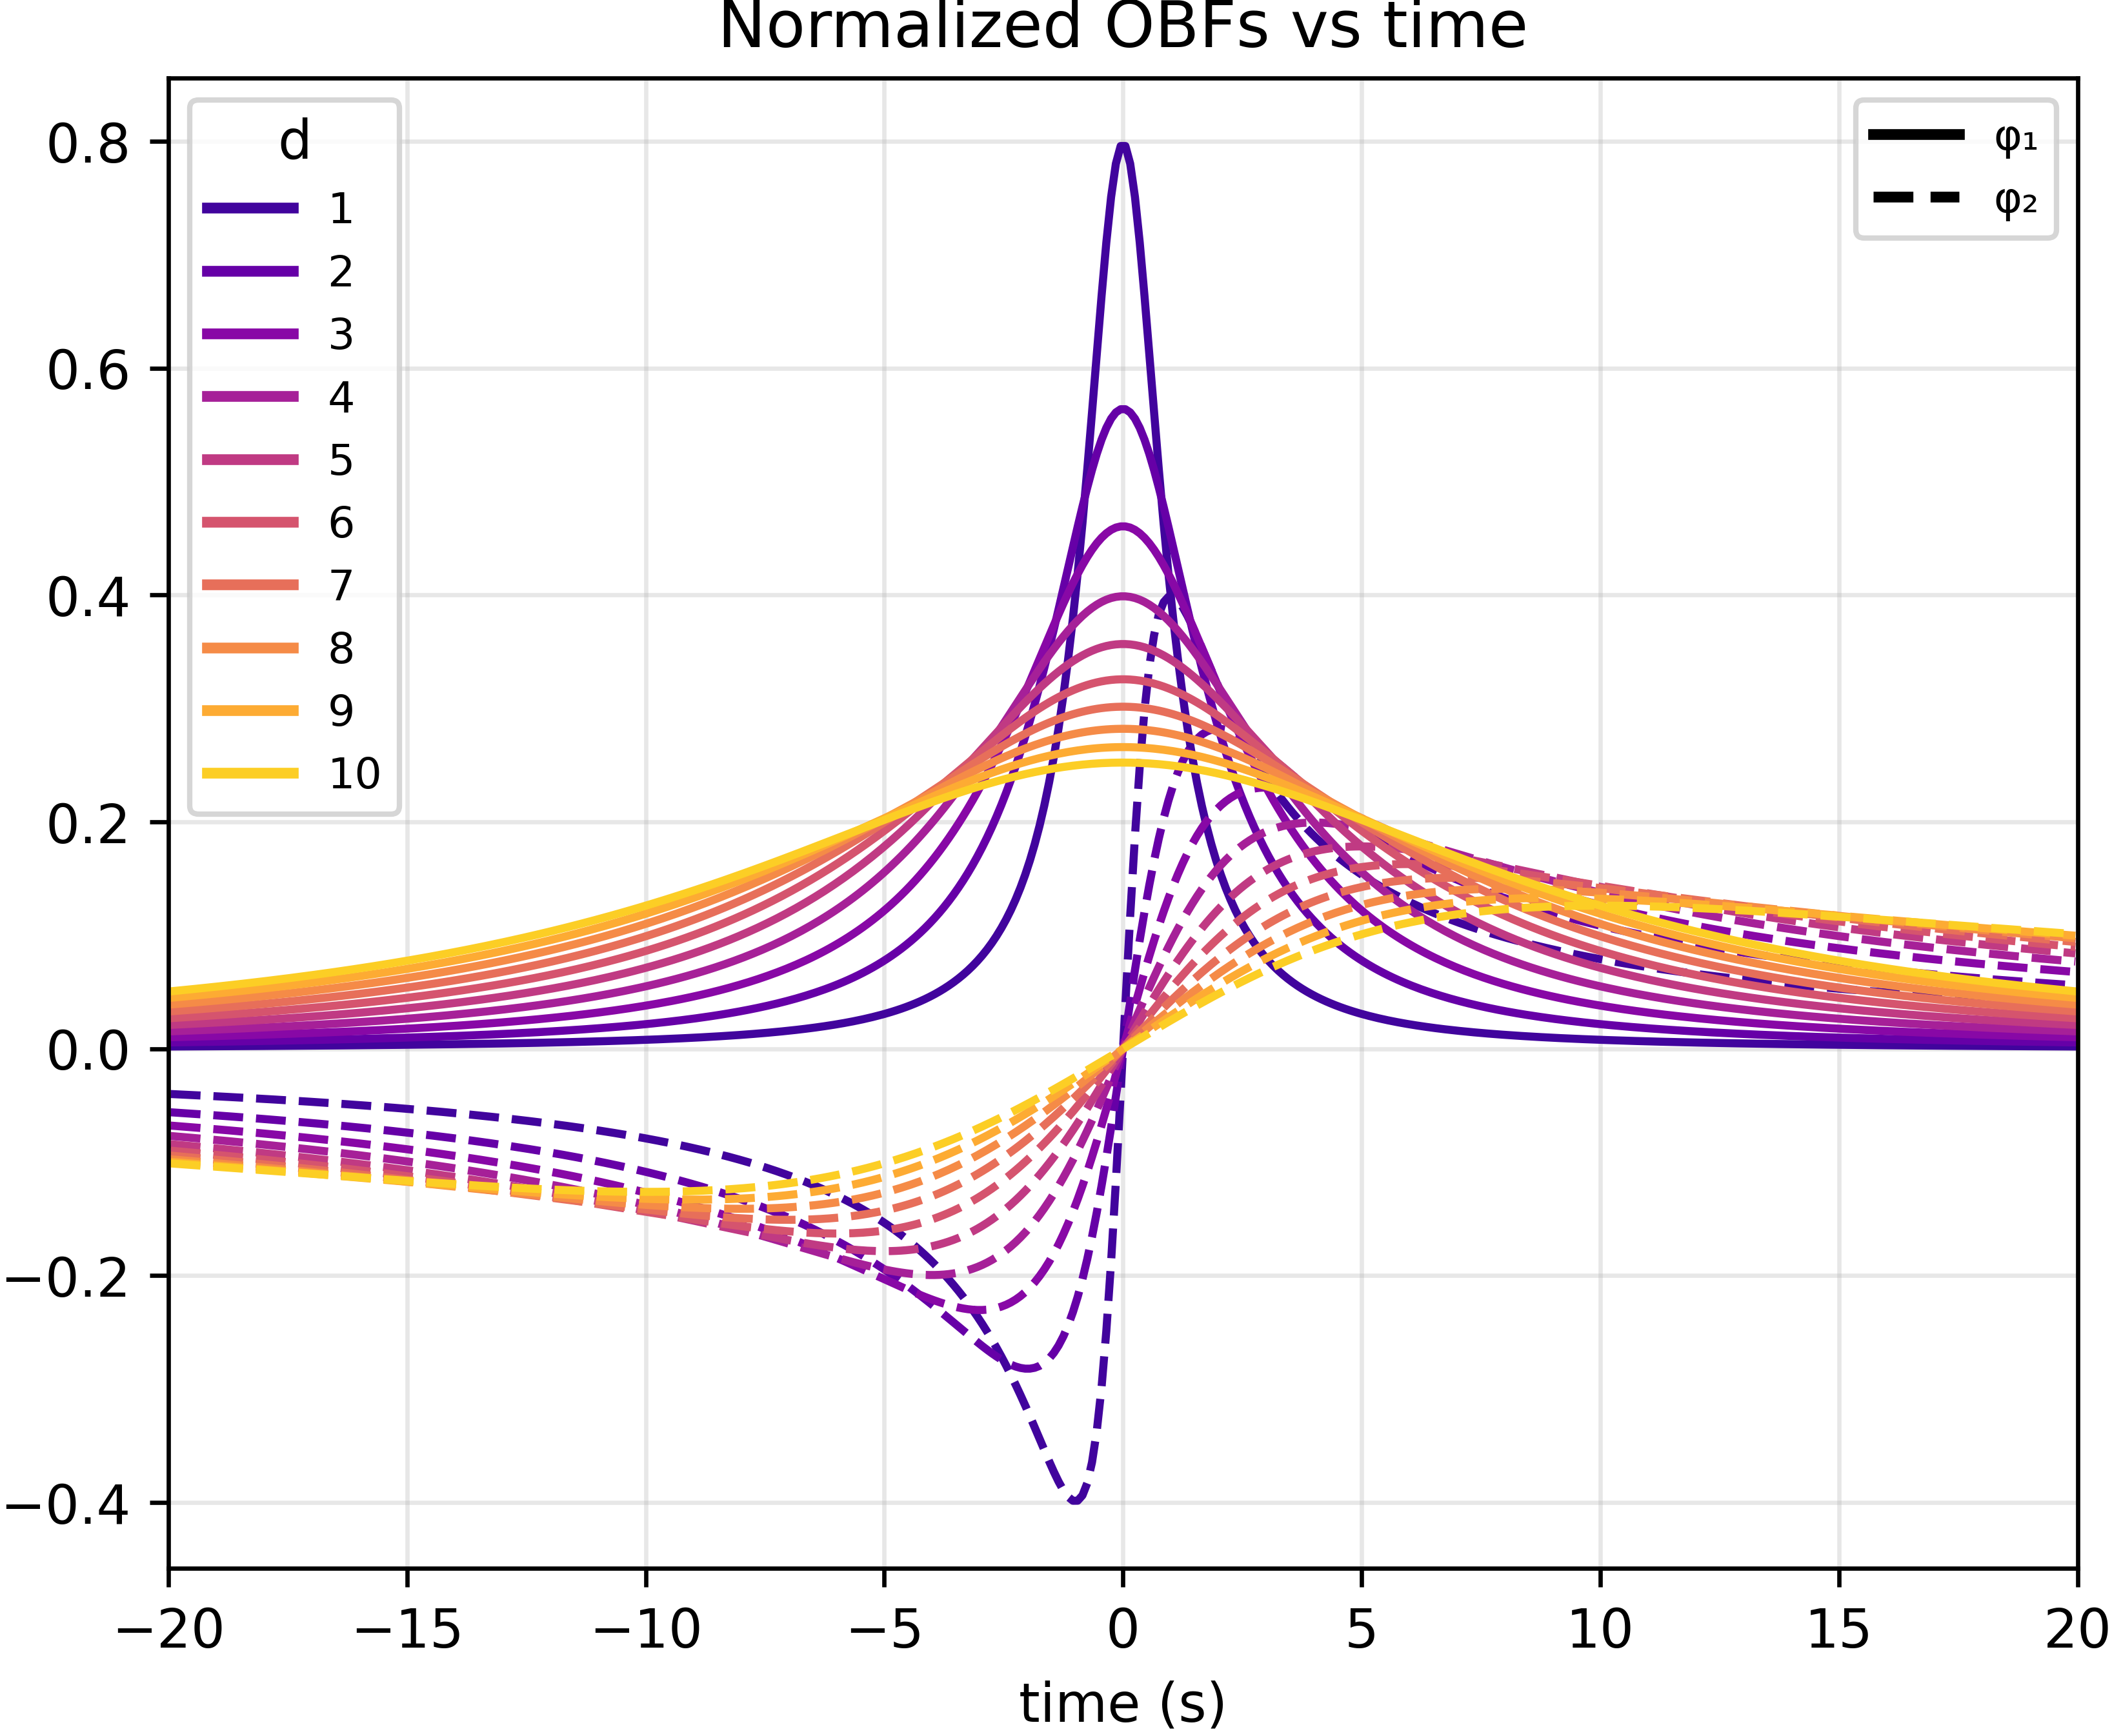
\includegraphics[width=\linewidth]{results_and_discus/figures/OBFs_d_time_normalized.png}
\end{minipage}

\vspace{0.5cm}

\begin{minipage}{0.75\linewidth}
\centering
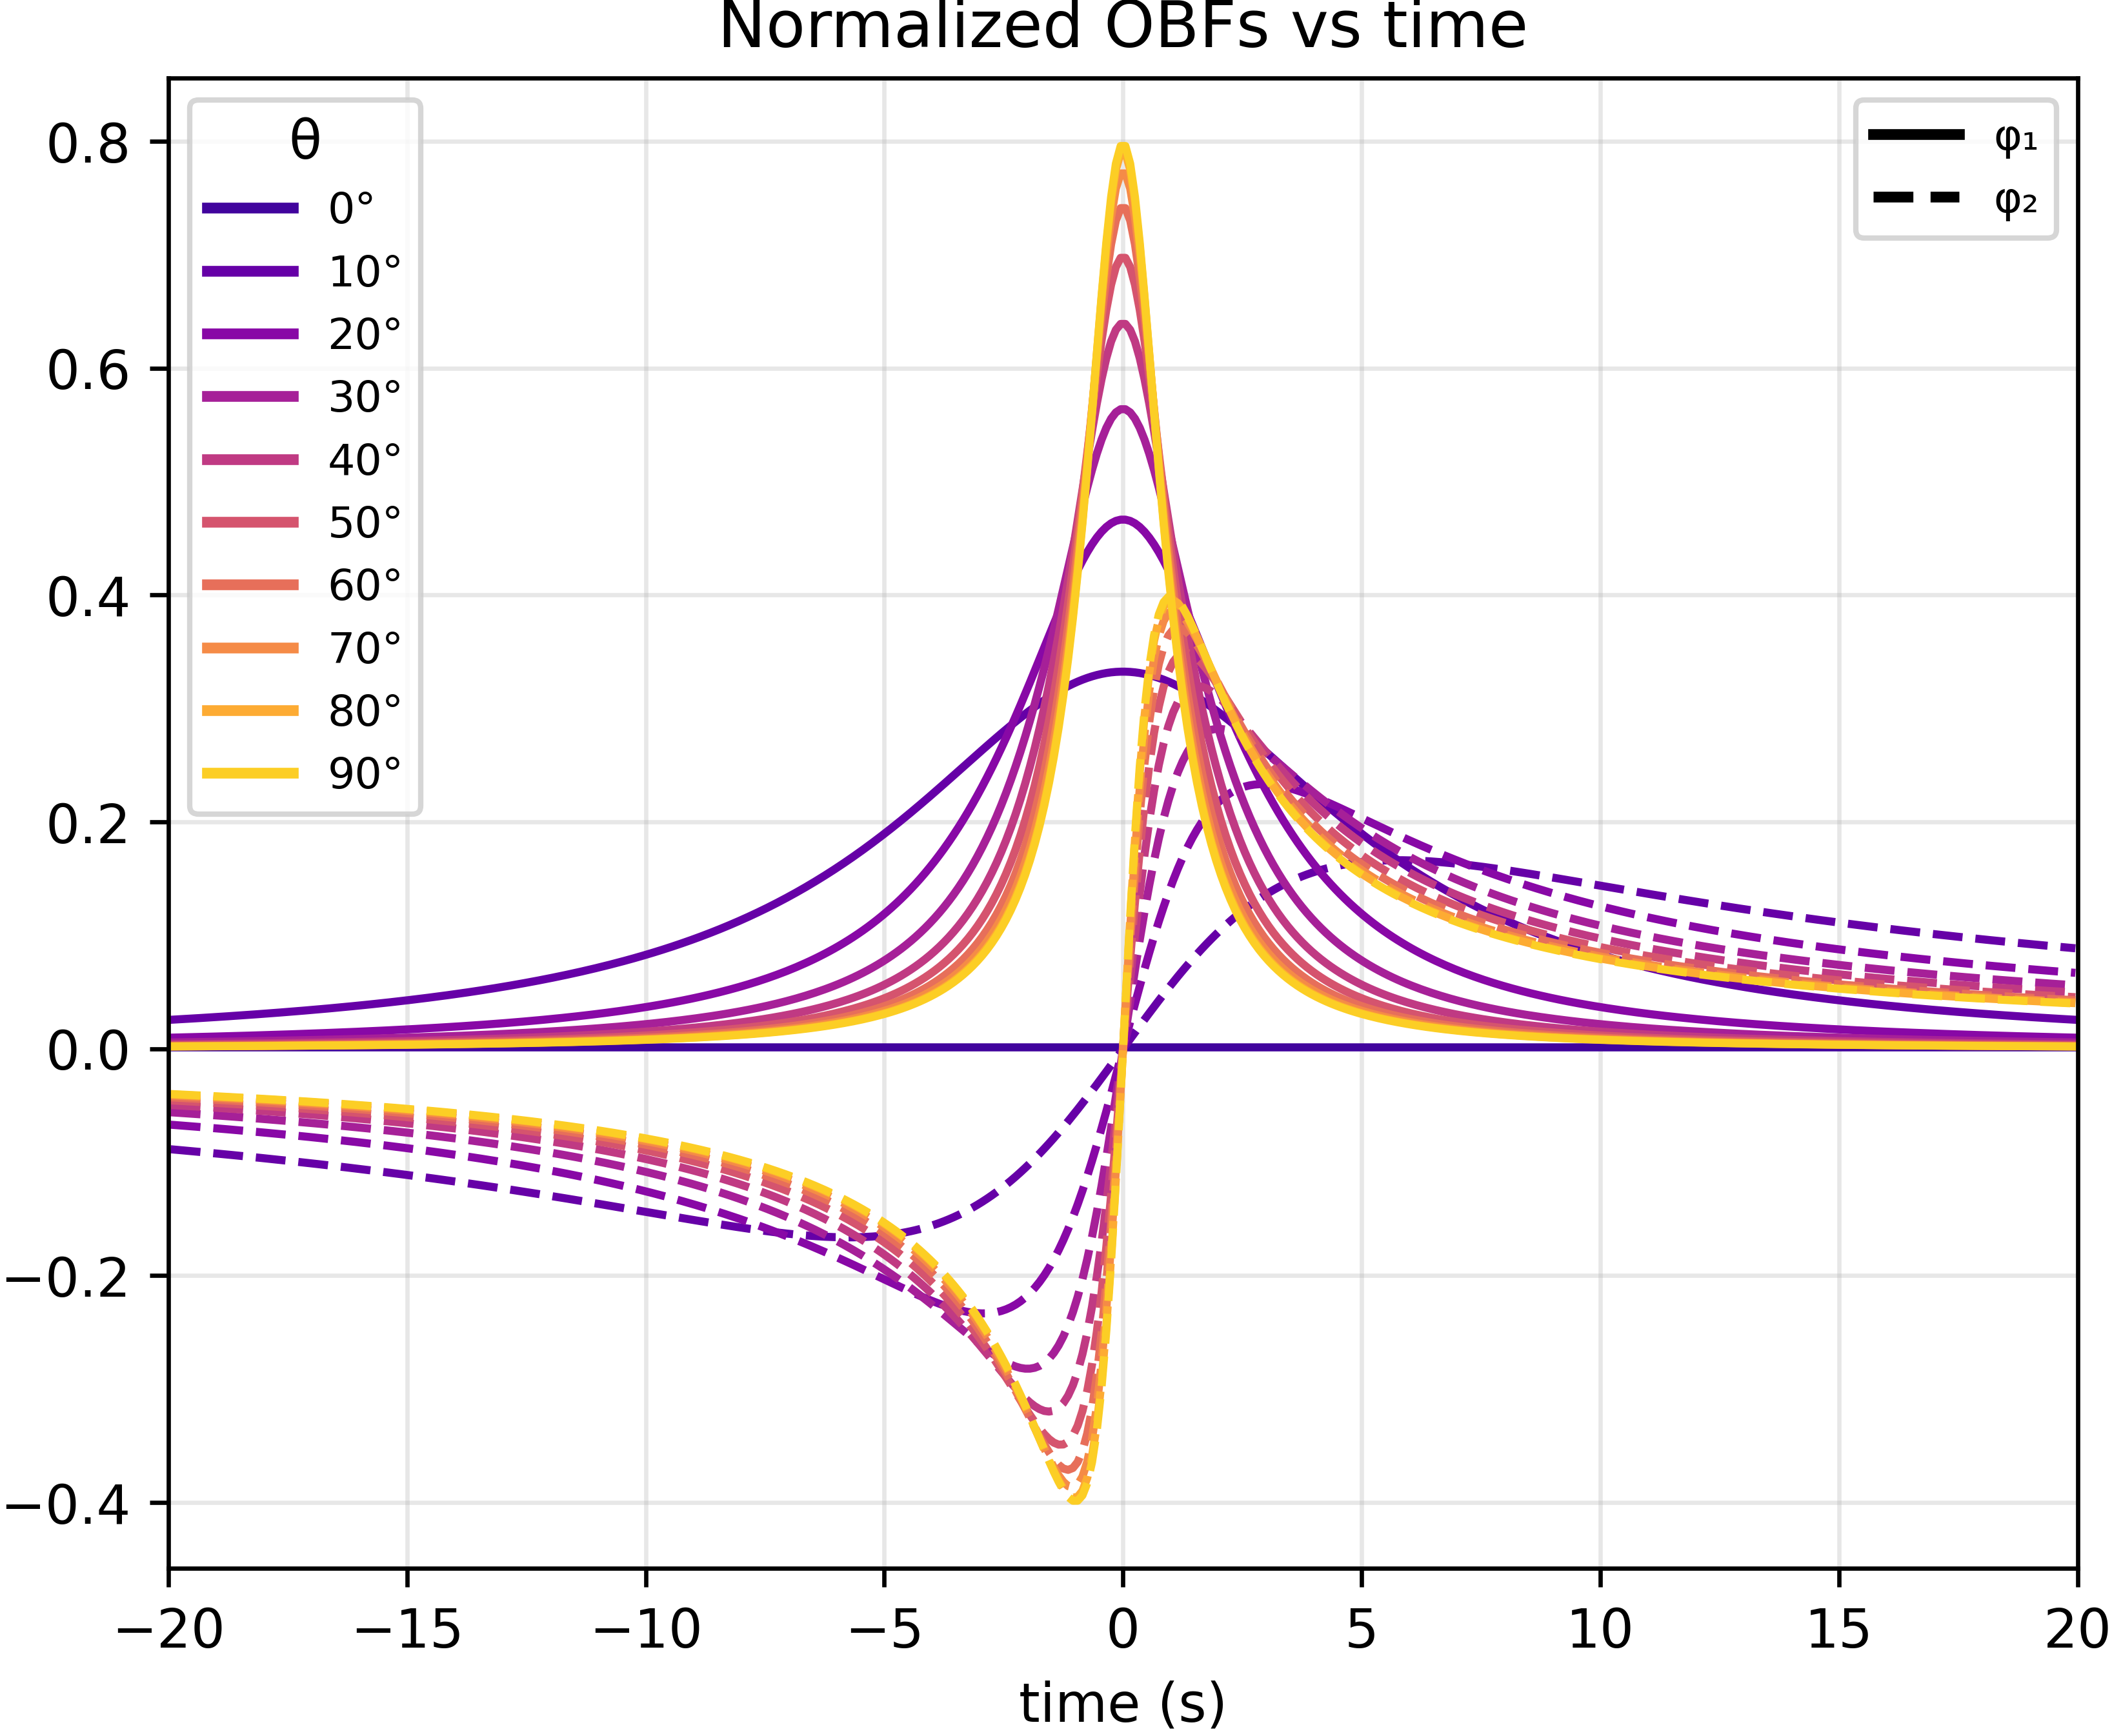
\includegraphics[width=\linewidth]{results_and_discus/figures/OBFs_theta_time_normalized.png}
\end{minipage}

\caption{Time-domain orthonormal basis functions $\Phi_1$ and $\Phi_2$, normalized over energy. Top: Influence of cable depth $d$ (with fixed $\theta = 90^\circ$). Bottom: Influence of trajectory angle $\theta$ (with fixed $d$ = 1).}
\label{fig:OBF_d_theta}
\end{figure}

Regarding cable OBF in isolation, it depends on two unknown parameters $(\frac{v}{d}, \theta)$ where we must assign a prior value for detection, analysis of the basis functions for varying values of $d$ and $\theta$ (see figure \ref{fig:OBF_d_theta}) indicates that their behavior exhibits relatively limited variation in the angular range from \(90^\circ\) to \(40^\circ\), whereas more pronounced changes occur between \(40^\circ\) and \(0^\circ\), a range that is less relevant for detection. This observation suggests a degree of robustness in the choice of the prior value for \(\theta\) before the detection stage. 
Regarding the parameter \(d\), its influence is consistent with that reported in Anderson’s formulation and in \cite{Otnes2007}. Specifically, a relatively large prior uncertainty in \(d\) is acceptable when the source–receiver distance is large. However, as the distance approaches \(\sim 3\,\text{m}\) (which coincides with our operational detection range), the choice of prior becomes increasingly critical, since beyond this threshold the basis functions exhibit pronounced distortion relative to the recorded waveform.


\subsection{Application conditions and Limitations}
Before ending, there are a couple of remarks regarding the extent to which the cable OBF are valid.

First, it is important to note that in Equation~\ref{eq:anomaly}, the first basis function is scaled by \(\cos\psi\). As a result, the projection of the signal onto $\Phi_1 $ vanishes as \(\Psi \rightarrow 90^\circ\), thereby reducing the effective dimensionality of the signal and potentially degrading detection performance in that orientation.

Second, the model assumes an infinitely straight conductor, but in reality it is only locally straight; as this study was never intended to discuss this aspect, it was encountered during the real experiment as the cable was not perfectly stretched (nor infinite), but no formulation or direct study has been made regarding this issue.

Third, the OBF are orthonormal in the continuous and unbounded time domain; in reality they are sampled, and only a finite portion is taken as templates. The effect was unnoticed during the experiments, as we have selected a large enough window with a sample rate that have negligible error on the orthonormality of the basis.